\documentclass[11pt,a4paper]{article}

\usepackage[margin=0.72in]{geometry}
\usepackage[T1]{fontenc}
\usepackage[utf8]{inputenc}
\usepackage{textcomp}
\IfFileExists{lmodern.sty}{\usepackage{lmodern}}{}
\usepackage{xcolor}
\usepackage{graphicx}
\usepackage{booktabs}
\usepackage{longtable}
\usepackage{array}
\usepackage{tabularx}
\usepackage{hyphenat}
\usepackage{xltabular}
\usepackage{siunitx}
\IfFileExists{lmodern.sty}{\usepackage{microtype}}{\usepackage[expansion=false,protrusion=false]{microtype}}
\usepackage[skins]{tcolorbox}
\usepackage{enumitem}
\usepackage{tikz}
\usepackage{multicol}
\usepackage{titlesec}
\usepackage{fancyhdr}
\usepackage{amsmath}
\usepackage{amssymb}
\usepackage[hidelinks]{hyperref}

% --- siunitx configuration forced to math-mode Omega to avoid W/M glyph bug ---
\sisetup{
  detect-all = true,
  per-mode=symbol,
  range-phrase=--,
  range-units=single,
  inter-unit-product=\ensuremath{\cdot}
}
\DeclareSIUnit{\ohmunit}{\ensuremath{\Omega}}

% Convenience macros that ALWAYS render Omega in math mode regardless of font
\newcommand{\ohmm}{\ensuremath{\,\Omega}}
\newcommand{\kohm}[1]{\ensuremath{#1\,\mathrm{k}\Omega}}
\newcommand{\Mohm}[1]{\ensuremath{#1\,\mathrm{M}\Omega}}
\newcommand{\Rohm}[1]{\ensuremath{#1\,\Omega}}

\setlength{\emergencystretch}{4em}
\sloppy


\usetikzlibrary{
arrows.meta,
positioning,
shapes.geometric,
shapes.misc,
calc,
fit,
matrix,
decorations.pathreplacing
}

% --------------------------------------------------------------------------
% Color theme
% --------------------------------------------------------------------------
\definecolor{EISNavy}{HTML}{153243}
\definecolor{EISBlue}{HTML}{1F6F8B}
\definecolor{EISTeal}{HTML}{1B998B}
\definecolor{EISMint}{HTML}{E8F4F2}
\definecolor{EISIce}{HTML}{EEF6FA}
\definecolor{EISAmber}{HTML}{B76E00}
\definecolor{EISAmberBG}{HTML}{FFF4DD}
\definecolor{EISRed}{HTML}{A33A3A}
\definecolor{EISRedBG}{HTML}{FCEAEA}
\definecolor{EISGreen}{HTML}{2E7D32}
\definecolor{EISGreenBG}{HTML}{EAF6EA}
\definecolor{EISGray}{HTML}{4B5563}
\definecolor{EISLightGray}{HTML}{F5F7FA}


\titleformat{\section}
{\Large\bfseries\color{EISNavy}}
{\thesection}{0.6em}{}
\titleformat{\subsection}
{\large\bfseries\color{EISBlue}}
{\thesubsection}{0.6em}{}
\titleformat{\subsubsection}
{\normalsize\bfseries\color{EISGray}}
{\thesubsubsection}{0.6em}{}

\pagestyle{fancy}
\setlength{\headheight}{14pt}
\fancyhf{}
\fancyhead[L]{EISight AD5933 Milk-EIS Prototype}
\fancyhead[R]{Final Blueprint v4.0c}
\fancyfoot[C]{\thepage}
\renewcommand{\headrulewidth}{0.4pt}

\setlist[itemize]{topsep=2pt,itemsep=2pt,leftmargin=1.3em}
\setlist[enumerate]{topsep=2pt,itemsep=2pt,leftmargin=1.5em}

\renewcommand{\arraystretch}{1.12}
\newcolumntype{Y}{>{\raggedright\arraybackslash}X}
\newcolumntype{L}[1]{>{\raggedright\arraybackslash}p{#1}}

% --------------------------------------------------------------------------
% Status macros
% --------------------------------------------------------------------------
\newcommand{\VALID}{\textcolor{EISGreen}{\textbf{VALID}}}
\newcommand{\VALIDCHANGES}{\textcolor{EISTeal}{\textbf{VALID WITH CHANGES}}}
\newcommand{\CORRECTION}{\textcolor{EISAmber}{\textbf{NEEDS CORRECTION}}}
\newcommand{\OPENRISK}{\textcolor{EISRed}{\textbf{OPEN RISK}}}
\newcommand{\OPENITEM}{\textcolor{EISRed}{\textbf{Open item:}}}
\newcommand{\ASSUMPTION}{\textcolor{EISAmber}{\textbf{Assumption:}}}
\newcommand{\CONFIRMEDtag}{\textcolor{EISGreen}{\textbf{Confirmed:}}}
\newcommand{\REVIEWER}{\textcolor{EISRed}{\textbf{Reviewer-risk warning:}}}

% --------------------------------------------------------------------------
% Boxes
% --------------------------------------------------------------------------
\newtcolorbox{verdictbox}{
enhanced, colback=EISIce, colframe=EISBlue, boxrule=0.8pt, arc=2mm,
left=2mm,right=2mm,top=1.5mm,bottom=1.5mm,
title=\textbf{Executive verdict}, coltitle=white, colbacktitle=EISBlue}

\newtcolorbox{riskbox}{
enhanced, colback=EISRedBG, colframe=EISRed, boxrule=0.8pt, arc=2mm,
left=2mm,right=2mm,top=1.5mm,bottom=1.5mm,
title=\textbf{Critical risk}, coltitle=white, colbacktitle=EISRed}

\newtcolorbox{rulebox}{
enhanced, colback=EISMint, colframe=EISTeal, boxrule=0.8pt, arc=2mm,
left=2mm,right=2mm,top=1.5mm,bottom=1.5mm,
title=\textbf{Frozen rule}, coltitle=white, colbacktitle=EISTeal}

\newtcolorbox{gatebox}{
enhanced, colback=EISGreenBG, colframe=EISGreen, boxrule=0.8pt, arc=2mm,
left=2mm,right=2mm,top=1.5mm,bottom=1.5mm,
title=\textbf{Go/no-go gate}, coltitle=white, colbacktitle=EISGreen}

\newtcolorbox{openbox}{
enhanced, colback=EISAmberBG, colframe=EISAmber, boxrule=0.8pt, arc=2mm,
left=2mm,right=2mm,top=1.5mm,bottom=1.5mm,
title=\textbf{Open item / clarify}, coltitle=white, colbacktitle=EISAmber}

\newtcolorbox{reviewerbox}{
enhanced, colback=EISRedBG, colframe=EISRed, boxrule=0.8pt, arc=2mm,
left=2mm,right=2mm,top=1.5mm,bottom=1.5mm,
title=\textbf{Reviewer-risk warning}, coltitle=white, colbacktitle=EISRed}

% --------------------------------------------------------------------------
% TikZ styles
% --------------------------------------------------------------------------
\tikzset{
eisblock/.style={draw=EISBlue, fill=EISIce, rounded corners=2pt, align=center,
  minimum height=8mm, text width=27mm, font=\small},
eisblockwide/.style={draw=EISBlue, fill=EISIce, rounded corners=2pt, align=center,
  minimum height=9mm, text width=35mm, font=\small},
eisgreen/.style={draw=EISGreen, fill=EISGreenBG, rounded corners=2pt, align=center,
  minimum height=8mm, text width=29mm, font=\small},
eiswarn/.style={draw=EISAmber, fill=EISAmberBG, rounded corners=2pt, align=center,
  minimum height=8mm, text width=27mm, font=\small},
eisrisk/.style={draw=EISRed, fill=EISRedBG, rounded corners=2pt, align=center,
  minimum height=8mm, text width=27mm, font=\small},
eisarrow/.style={-{Latex[length=2.4mm]}, thick, draw=EISNavy},
eisdashed/.style={-{Latex[length=2.4mm]}, thick, dashed, draw=EISGray},
eissmall/.style={draw=EISGray, fill=EISLightGray, rounded corners=2pt, align=center,
  minimum height=6mm, text width=24mm, font=\scriptsize}
}

% --------------------------------------------------------------------------
% Title
% --------------------------------------------------------------------------
\title{\textbf{\color{EISNavy}Final Audited Technical Blueprint and Laboratory Manual for an AD5933-Based Milk-Adulteration EIS Prototype} \\[4pt] \large Blueprint v4.0c --- frozen lab authority (procedural-patch revision)}
\author{EISight Laboratory Master Document}
\date{Builds on v4.0b. Adds: G-RFB SSOP-probing safety caution, lab-DMM cross-check promoted to a pre-G-SAT step, JSONL examples brought into line with the 5--100\,kHz default, and an explicit note that G-SAT and G-LIN are analyses applied to the F.10 resistor-sweep dataset rather than separate sweep sessions.}

\begin{document}
\maketitle
\begin{center}
\begin{tabularx}{0.94\textwidth}{
>{\raggedright\arraybackslash}p{35mm}
>{\raggedright\arraybackslash}X
}
\toprule
\textbf{Project direction} &
Milk-first, calibration-first, fixed-geometry two-electrode EIS prototype using AD5933 module, ESP32 control, DS18B20 temperature logging, and laptop-side processing.\\

\textbf{Current hardware state} &
Two AD5933 modules DMM-verified unpowered: J1 open ($\approx\Mohm{3}$), J2 closed ($\approx\Rohm{0}$), J3 open, J4 open, J5 open, J6 closed. Both are in vendor-defined Direct mode.\\

\textbf{Primary hardware decision} &
Preserve one module in Direct mode as a control after Direct-mode sanity passes. Convert the other module to Dual-op-amp mode \emph{after} both boards have been power-, $\mathrm{I^2C}$-, and single-resistor-tested in their as-received state.\\

\textbf{Evidence basis} &
Official AD5933 data sheet, official AD5933 evaluation-board guide (UG-364), vendor module user manual (partially trusted; pages 1--5 only), project DMM measurements, uploaded board photographs, Taobao purchase audit, EISight progress report, and existing EISight pipeline source.\\
\bottomrule
\end{tabularx}
\end{center}
\vspace{2mm}

\begin{rulebox}
This document is deliberately conservative. It is not a marketing plan. It is a bench-executable engineering and publication-risk control document. Any dataset collected before the jumper-state issue, Direct-mode sanity, rework verification, resistor characterization, DC-bias check, cell repeatability, temperature logging, and cleaning/QC gates are closed must be treated as exploratory only.
\end{rulebox}

\vspace{2mm}

\begin{tcolorbox}[enhanced, colback=EISIce, colframe=EISNavy, boxrule=0.8pt, arc=2mm,
  left=2mm,right=2mm,top=1.5mm,bottom=1.5mm,
  title=\textbf{v4.0b Technical Patch Summary (what changed since v4.0)},
  coltitle=white, colbacktitle=EISNavy]
This revision keeps the v4.0 architecture and BOM intact and patches only the items where official AD5933 documentation, datasheet specifications, or basic physics required correction. The patches are:
\begin{enumerate}[topsep=2pt,itemsep=1pt,leftmargin=1.4em]
\item \textbf{DC-bias gate is now a three-measurement procedure (Section~\ref{sec:E}.11):} log $V_{DC}(P1\!-\!\mathrm{GND})$, $V_{DC}(P2\!-\!\mathrm{GND})$, and $V_{DC}(P1\!-\!P2)$. Primary pass/fail is on the differential $|V_{DC}(P1\!-\!P2)|<\SI{50}{\milli\volt}$ under active excitation, with both no-load and \Rohm{470}-loaded conditions. Absolute values retained as diagnostics.
\item \textbf{AC-coupling capacitor sizing and placement (Section~\ref{sec:E}.11, \ref{sec:H}.6):} if added, minimum \SI{10}{\micro\farad} non-polar, \SI{47}{\micro\farad} film preferred, in series with VOUT \emph{upstream} of the DPDT common terminal so it is present in both CAL and SAMPLE paths and is absorbed by the per-frequency gain factor. Calibrate through.
\item \textbf{$R_{FB}$ inventory gate (new, Section~\ref{sec:F}.4):} DMM-measure resistance between AD5933 Pin~4 ($R_{FB}$) and Pin~5 (VIN) on each module with the IC unpowered, before any wet test. Logged in \texttt{hardware/rfb\_inventory.csv}.
\item \textbf{Saturation/clipping characterization gate (G-SAT, Section~\ref{sec:F}.10):} explicit resistor-sweep check that the AD5933 + on-board $R_{FB}$ does not saturate the internal ADC at expected milk impedances ($\Rohm{330}$--$\Rohm{700}$). $R_{FB}$ rework or external buffer (per AD5933 datasheet Fig.~35) is conditional on this gate failing -- not pre-emptive.
\item \textbf{Amplitude-linearity gate (G-LIN, Section~\ref{sec:F}.10):} repeat one resistor at Range~2 versus Range~4 and require calibrated $|Z|$ agreement within 2\%.
\item \textbf{Conservative initial trusted band (Section~\ref{sec:H}.5):} 5--100\,kHz with internal MCLK; below 5\,kHz only after explicit resistor QC validation, per UG-364, p.~19, on internal-oscillator spectral leakage. External MCLK at \SI{4}{\mega\hertz} is reclassified as an \emph{optional fallback}, not a mandatory addition.
\item \textbf{Range~4 rationale corrected (Section~\ref{sec:H}.6):} Range~4 minimizes the AC perturbation amplitude (linearity-friendly) but does \emph{not} minimize the DC differential $V(P1\!-\!P2)$ in raw Direct mode, because VIN is hard-biased at $V_{DD}/2$ \cite{ad5933ds}. AC coupling or Dual-op-amp-mode buffering is the only mechanism that drives the differential toward zero independently of range. The previous v4.0 wording is corrected.
\item \textbf{Signed int16 register parsing (Sections~\ref{sec:I}.2, I.4, I.5):} the AD5933 stores real (\texttt{0x94}/\texttt{0x95}) and imaginary (\texttt{0x96}/\texttt{0x97}) results in twos-complement 16-bit format \cite{ad5933ds}. Firmware and pipeline must perform sign-extending parsing. The internal temperature register is 14-bit signed in a 16-bit envelope.
\item \textbf{Quiescent current rule relaxed (Section~\ref{sec:F}.4):} 15--25\,mA is treated as a reference expectation, not a hard fail. Hard-fail is reserved for thermal runaway, unstable 3.3\,V rail, large module-to-module mismatch ($>$50\%), I\textsuperscript{2}C bus failure, or visible/smell damage.
\item \textbf{Risk register additions (Section~\ref{sec:K}.2):} new rows for TIA/$R_{FB}$ saturation, low-frequency DFT spectral leakage, and AC-coupling calibration-path leak.
\end{enumerate}

The patches do \emph{not} require a different BOM, a different cell, a different ESP32 firmware architecture, or a different paper scope. They tighten the validity gates between Day-B0 sanity and first-liquid testing.

The single biggest operational change is point~6: the publication-candidate trusted band is now \textbf{5--100\,kHz} until resistor QC at lower frequencies is recorded.
\end{tcolorbox}

\vspace{2mm}

\begin{tcolorbox}[enhanced, colback=EISIce, colframe=EISNavy, boxrule=0.8pt, arc=2mm,
  left=2mm,right=2mm,top=1.5mm,bottom=1.5mm,
  title=\textbf{v4.0c Procedural Patch Summary (changes since v4.0b)},
  coltitle=white, colbacktitle=EISNavy]
v4.0c is a small procedural revision. The architecture, BOM, gates, and acceptance criteria of v4.0b are preserved. The patches address an external review finding that:
\begin{enumerate}[topsep=2pt,itemsep=1pt,leftmargin=1.4em]
\item \textbf{G-SAT and G-LIN are analyses applied to the F.10 resistor-sweep dataset, not separate sweep sessions.} The text in F.10.a / F.10.b is reworded to make this explicit, removing any ambiguity that could lead to redundant data acquisition.
\item \textbf{G-RFB SSOP-probing safety caution (Section~\ref{sec:F}.4):} direct DMM probing of AD5933 Pin~4 / Pin~5 is correct in principle but mechanically risky on a 0.65\,mm SSOP package. If safe probing cannot be achieved with a magnifier and fine probes, do not force it; G-SAT will resolve the saturation question empirically.
\item \textbf{Lab-DMM cross-check on \kohm{1} promoted to a pre-G-SAT step (Section~\ref{sec:F}.7):} the gain factor is anchored on \texttt{R1k\_01}, so any handheld-DMM error in that single measurement propagates through every calibrated $|Z|$ figure. The cross-check is moved from ``before publication'' (Open Items) to ``before resistor characterization.''
\item \textbf{JSONL example (Section~\ref{sec:I}.4) brought into line with the new default sweep band:} \texttt{start\_hz} updated from \SI{1000}{\hertz} to \SI{5000}{\hertz}, \texttt{points} from 100 to 96. This eliminates a silent drift between the firmware example and the v4.0b trusted-band rule.
\end{enumerate}
No bench-procedure changes, no new gates, no new components. v4.0c is what you should follow on the bench.
\end{tcolorbox}

\tableofcontents
\newpage

% ==========================================================================
\section{SECTION A --- Executive verdict}
\label{sec:A}

\begin{verdictbox}
The current project direction is technically sound \textbf{only if the instrument is treated as an unvalidated measurement system until resistor, liquid-cell, DC-bias, and repeatability gates are passed}. The AD5933+ESP32+laptop architecture is feasible with the confirmed hardware, but both AD5933 modules are currently in Direct mode. That means the onboard AD8606 is physically present but is bypassed in the main sample path. For milk-range impedances, this is the highest immediate hardware risk.

The project is currently paper-capable at the \textbf{class project / AURA demonstration} level after basic resistor and pure-milk repeatability. It can become an \textbf{undergraduate or regional IEEE-style conference paper} if calibration, repeatability, temperature control, and controlled adulteration data are clean. It is not yet strong-indexed-conference or journal-ready until external/reference-instrument comparison, multi-day grouped validation, cell-to-cell reproducibility, blind samples, and uncertainty reporting are added.
\end{verdictbox}

\subsection{A.1 Technical soundness}

\begin{itemize}
\item \textbf{Sound core:} AD5933 impedance conversion, ESP32 control, fixed cell, DS18B20 temperature logging, and laptop-side calibration/QC is the correct reduced-scope execution path.
\item \textbf{Main correction:} The DMM continuity results now overrule earlier assumptions. Both modules are currently in Direct mode, not Dual-op-amp mode.
\item \textbf{Immediate action:} First, verify both modules power up, respond on $\mathrm{I^2C}$, and produce sane data on a single $\kohm{1}$ resistor in their as-received Direct mode. \emph{Only then} rework Module B to Dual-op-amp mode. Module A remains Direct as the comparison reference.
\end{itemize}

\subsection{A.2 Realistic feasibility with confirmed hardware}

\begin{itemize}
\item \textbf{Feasible:} Yes, for a laptop-in-the-loop prototype that measures calibrated resistor loads, a fixed SS316L two-electrode cell, DI-water blank behavior, and milk spectra.
\item \textbf{Not yet proven:} Reliable milk-adulteration classification. The simulator and ML pipeline do not prove the instrument works.
\item \textbf{Most likely first success:} Resistor sweep repeatability, followed by pure-milk repeatability over a narrow trusted frequency band.
\item \textbf{Most likely first failure:} Low-impedance milk loads causing poor accuracy, phase instability, or saturation if the AFE is not actually active after rework; or electrolysis at the SS316L electrodes if a DC bias leaks through the cell (see Section~\ref{sec:E} DC-bias gate).
\end{itemize}

\subsection{A.3 Paper-worthiness today}

\begin{xltabular}{\textwidth}{L{42mm}L{38mm}Y}
\toprule
\textbf{Venue level} & \textbf{Current verdict} & \textbf{What must be added}\\
\midrule
Class project / AURA demonstration &
Achievable after first stable resistor and pure milk plots. &
Resistor calibration, repeatable pure milk spectra, clear system diagram, honest limitations.\\
Undergraduate conference / local conference &
Achievable if data collection is disciplined. &
Multi-day pure/adulterated dataset, QC rejection rules, grouped validation, temperature metadata, cell cleaning SOP.\\
Strong indexed conference &
Possible but not guaranteed. &
Reference instrument or high-quality LCR cross-check, cell-to-cell reproducibility, blind samples, ablations, confidence intervals.\\
Journal &
Not supported at today's state. &
Larger sample size, independent ground truth, reference-lab comparison, uncertainty budget, robust external validation, stronger novelty than ``low-cost EIS works''.\\
\bottomrule
\end{xltabular}

\subsection{A.4 Main blockers to publication-quality work}

\begin{riskbox}
\begin{enumerate}
\item Both AD5933 modules are confirmed in Direct mode; the AD8606 path is not yet validated in the active sample path.
\item Direct-mode DC-bias at the electrodes is not yet measured and is a latent electrolysis risk for SS316L in milk.
\item No resistor-based trusted-band map exists yet.
\item No verified fixed SS316L cell geometry exists yet.
\item No cross-session pure-milk repeatability has been demonstrated.
\item No reference instrument comparison exists.
\item No grouped-by-day validation dataset exists.
\item No blind-sample protocol exists.
\item DMM accuracy class is not yet recorded; 0.1\% resistors cannot be claimed beyond the DMM's own accuracy.
\end{enumerate}
\end{riskbox}

\subsection{A.5 Immediate highest-risk issue}

\begin{reviewerbox}
A reviewer will not accept ``AD5933 module with AD8606'' as evidence that the AFE improved low-impedance measurement. The only acceptable answer is a resistor characterization plot comparing Direct mode and Dual-op-amp mode on the same resistor set, showing the trusted frequency band and residual errors, measured with the same DMM-metrology calibration values on both modules.
\end{reviewerbox}

% ==========================================================================
\section{SECTION B --- Full technical audit and validation}
\label{sec:B}

\subsection{B.1 Audit matrix}

\small
\begin{xltabular}{\textwidth}{L{38mm}L{32mm}Y}
\toprule
\textbf{Item} & \textbf{Verdict} & \textbf{Audit decision}\\
\midrule
\endfirsthead
\toprule
\textbf{Item} & \textbf{Verdict} & \textbf{Audit decision}\\
\midrule
\endhead

Overall architecture & \VALIDCHANGES & AD5933 + ESP32 + fixed cell + DS18B20 + laptop processing is the right reduced-scope architecture. Treat it as a calibrated instrument, not a generic ML sensor.\\
Signal chain & \VALIDCHANGES & Correct only after Module B is converted and validated. Current Direct mode leaves the low-impedance milk path under-defended.\\
AD5933 module choice & \VALIDCHANGES & The module is usable, but the AD5933 native range is not ideal for low-impedance milk. The data sheet gives the standard range as \kohm{1}--\Mohm{10} and says \Rohm{100}--\kohm{1} requires additional circuitry \cite{ad5933ds}. The onboard AD8606 path must be activated and characterized.\\
Confirmed Direct-mode jumper state & \VALID & DMM measurement is now the source of truth: J1 open, J2 closed, J3 open, J4 open, J5 open, J6 closed on both modules. This matches the vendor manual's Direct-mode rule \cite{vendorManual}.\\
Onboard AD8606 significance & \VALIDCHANGES & AD8606 is physically present but is \emph{expected to be bypassed} in the main sample path per the vendor's Direct-mode jumper convention. The bypass is verified empirically by Direct-vs-Dual resistor characterization (G-SAT, G-LIN, full F.10 map). Its exact topology after rework remains an \OPENRISK{} until that characterization is complete.\\
Need to convert one board to Dual-op-amp mode & \VALID & Required before primary milk testing. One Direct module and one Dual-op-amp candidate, not both Direct and not both reworked.\\
\textbf{Bench-order rule} & \VALID & Power + $\mathrm{I^2C}$ sanity on \emph{both} modules in Direct mode \emph{before} any rework, using a single \kohm{1} sweep as a functional check. This prevents rework from masking vendor-side defects.\\
ESP32 role & \VALID & $\mathrm{I^2C}$ to AD5933, 1-Wire to DS18B20, USB serial to laptop. No final calibration, ML, dashboarding, or cloud logic in v1.\\
DS18B20 role & \VALIDCHANGES & Read sample temperature before and after sweep only; no 1-Wire activity during AD5933 conversion. Log probe ROM ID and pre/post temperature. AD5933 internal temperature register is logged as board/die temperature only.\\
Manual CAL/SAMPLE switching & \VALID & Preferred over analog muxes for v1. Switch only while AD5933 is idle. Switch state is metadata.\\
Cell material and geometry & \VALIDCHANGES & Fixed-geometry direct-contact cell is correct. Geometry remains v1 candidate until DI-water blank, pure milk repeatability, and calibration gates pass.\\
SS316L vs SS304 & \CORRECTION & SS304 is mockup-only. SS316L is the final electrode material. SS316L is in transit from China (ETA $\approx$ 1--2 weeks). Authenticity remains an open item.\\
Power architecture & \VALIDCHANGES & Use simple USB/laptop-in-loop power first. Do not redesign power until resistor data show a noise problem. Common ground is mandatory. See Section~\ref{sec:C} for the power discipline rules.\\
Calibration resistor strategy & \VALIDCHANGES & 0.1\% resistor set (\Rohm{100}, \Rohm{330}, \Rohm{470}, \kohm{1}, \kohm{4.7}, \kohm{10}) is well chosen, but DMM accuracy limits the claim: record DMM model and accuracy class; if DMM is worse than 0.1\% the reported metrology is DMM-limited.\\
Shielding/interconnect strategy & \CORRECTION & Module SMA connectors are DDS-OUT and EXT-CLK, not the sample path. Sample path is Vin/Vout pads/terminals. Use short twisted pair (first approach) or shielded coax with deliberate single-end shield grounding.\\
\textbf{DC bias at electrodes (v4.0b)} & \OPENRISK & The receive stage VIN is hard-biased at $V_{DD}/2 \approx \SI{1.65}{\volt}$ \cite{ad5933ds}; the transmit stage VOUT carries a per-range DC bias (Range~1: \SI{1.48}{\volt}, Range~4: \SI{0.173}{\volt}). The differential across a load connected directly between VOUT and VIN is therefore non-zero in every range, with Range~4 giving the \emph{largest} differential ($\approx\SI{1.48}{\volt}$) and Range~1 the smallest ($\approx\SI{0.17}{\volt}$). Either AC coupling or Dual-op-amp-mode buffering is required to drive the differential below \SI{50}{\milli\volt}. Settled empirically by G-DC3 (Section~\ref{sec:E}.11).\\
\textbf{Excitation range selection (v4.0b)} & \VALIDCHANGES & Default for milk: Range~4 (\SI{198}{\milli\volt\,pp}). Rationale is \emph{linearity}, not electrolysis: small AC perturbation keeps the system in its small-signal linear regime. Electrolysis is gated separately via G-DC3. Range escalation requires G-DC3 + G-LIN agreement at the new range.\\
\textbf{TIA / $R_{FB}$ saturation (v4.0b NEW)} & \OPENRISK & On-board $R_{FB}$ value on the Chinese clone is unpublished. EVAL-AD5933EBZ default is \kohm{200}; Ibba uses selectable \Rohm{200}--\kohm{200}. For \Rohm{330} milk at Range~4 with \kohm{20} $R_{FB}$, $V_\mathrm{ADC}\approx\SI{12}{\volt}$ and the receive stage saturates. Settled by G-RFB (DMM measurement) plus G-SAT (resistor-sweep clipping signature).\\
\textbf{Low-frequency DFT leakage (v4.0b NEW)} & \OPENRISK & Internal MCLK + $f_\mathrm{exc}<\SI{5}{\kilo\hertz}$ does not capture an integer number of periods in the 1024-sample window \cite{ug364}. Per-frequency calibration partially absorbs this. Initial trusted band restricted to \SIrange{5}{100}{\kilo\hertz}; sub-5\,kHz on resistor QC validation only.\\
\textbf{Signed-int16 register parsing (v4.0b NEW)} & \CORRECTION & AD5933 real/imag/temperature registers are twos-complement \cite{ad5933ds}. Mandatory firmware and pipeline parsing rule (Section~\ref{sec:I}.2.a).\\
Parasitic fixture characterization (new) & \VALIDCHANGES & Open, short, and cable-motion checks are mandatory before resistor characterization. Without these, residual fixture parasitics are indistinguishable from real cell impedance.\\
Software pipeline & \VALIDCHANGES & Add session calibration, trusted-band selection, QC, metadata, temperature handling, and grouped validation before real claims.\\
Dataset collection logic & \CORRECTION & No adulteration data until pure milk repeatability is proven. Data grouped by day, milk source/brand, cell, operator, and calibration session.\\
Repeatability plan & \VALIDCHANGES & Within-session, cross-session, cell-to-cell, and cleaning/carryover blanks. Pure milk repeatability is the real v1 milestone.\\
Statistical validation plan & \OPENRISK & Day-grouped cross-validation, blind holdout, confidence intervals, ablations. Avoid random row splits.\\
Publication feasibility & \VALIDCHANGES & Feasible as a disciplined prototype study. Novelty must be conservative.\\
\bottomrule
\end{xltabular}
\normalsize

\subsection{B.2 Audit summary}

\begin{rulebox}
The master architecture is frozen, but the measurement system is not yet validated. The next defensible scientific step is not milk adulteration. It is: (1) Direct-mode power/$\mathrm{I^2C}$/\kohm{1} sanity on both boards, (2) rework of Module B, (3) post-rework sanity on Module B, (4) DC-bias verification at the electrode pads on both modules, (5) full resistor characterization Direct vs Dual-op-amp, (6) pure-liquid repeatability.
\end{rulebox}

% ==========================================================================
\section{SECTION C --- Frozen final system architecture}
\label{sec:C}

\subsection{C.1 Frozen architecture statement}

\begin{itemize}
\item \textbf{Module A:} \texttt{AD5933-A-DIRECT}. Keep in Direct mode. Use for control/comparison and fallback.
\item \textbf{Module B:} \texttt{AD5933-B-DUAL-AFE}. Convert to Dual-op-amp mode \emph{only after} Direct-mode sanity passes on both modules.
\item \textbf{Controller:} ESP32-DevKitC-32E. Controls AD5933 and temperature probes; streams raw data to laptop.
\item \textbf{Processing:} Laptop Python/Streamlit. Performs calibration, QC, feature extraction, model training, inference.
\item \textbf{Cell:} Fixed-geometry SS316L two-electrode cell. SS304 excluded from final data.
\item \textbf{Switching:} Manual CAL/SAMPLE; no analog mux in v1.
\end{itemize}

\begin{figure}[!ht]
\centering
\resizebox{0.96\textwidth}{!}{%
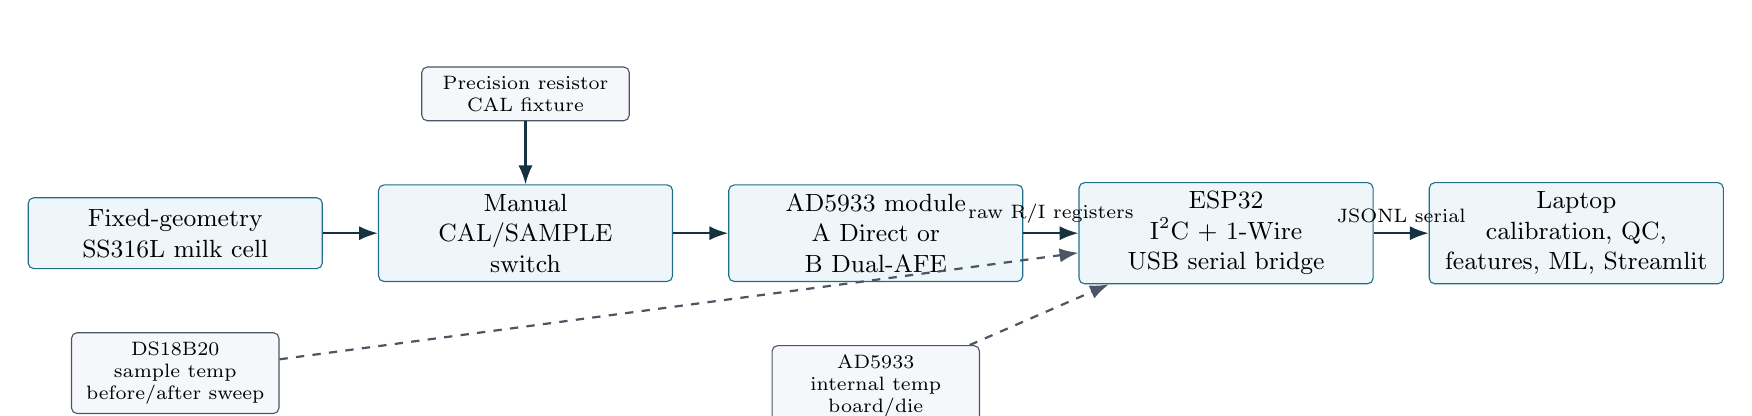
\begin{tikzpicture}[node distance=8mm and 7mm]
\node[eisblockwide] (cell) {Fixed-geometry\\SS316L milk cell};
\node[eisblockwide, right=of cell] (cal) {Manual\\CAL/SAMPLE\\switch};
\node[eisblockwide, right=of cal] (ad) {AD5933 module\\A Direct or B Dual-AFE};
\node[eisblockwide, right=of ad] (esp) {ESP32\\$\mathrm{I^2C}$ + 1-Wire\\USB serial bridge};
\node[eisblockwide, right=of esp] (lap) {Laptop\\calibration, QC, features, ML, Streamlit};
\node[eissmall, below=of cell] (temp) {DS18B20\\sample temp\\before/after sweep};
\node[eissmall, below=of ad] (die) {AD5933\\internal temp\\board/die};
\node[eissmall, above=of cal] (res) {Precision resistor\\CAL fixture};

\draw[eisarrow] (cell) -- (cal);
\draw[eisarrow] (res) -- (cal);
\draw[eisarrow] (cal) -- (ad);
\draw[eisarrow] (ad) -- node[above,font=\scriptsize]{raw R/I registers} (esp);
\draw[eisarrow] (esp) -- node[above,font=\scriptsize]{JSONL serial} (lap);
\draw[eisdashed] (temp) -- (esp);
\draw[eisdashed] (die) -- (esp);
\end{tikzpicture}
}
\caption{Full system architecture. The laptop, not the ESP32, is the calibration and inference authority.}
\label{fig:system_arch}
\end{figure}

\subsection{C.2 Power tree and discipline}

\begin{figure}[!ht]
\centering
\resizebox{0.85\textwidth}{!}{%
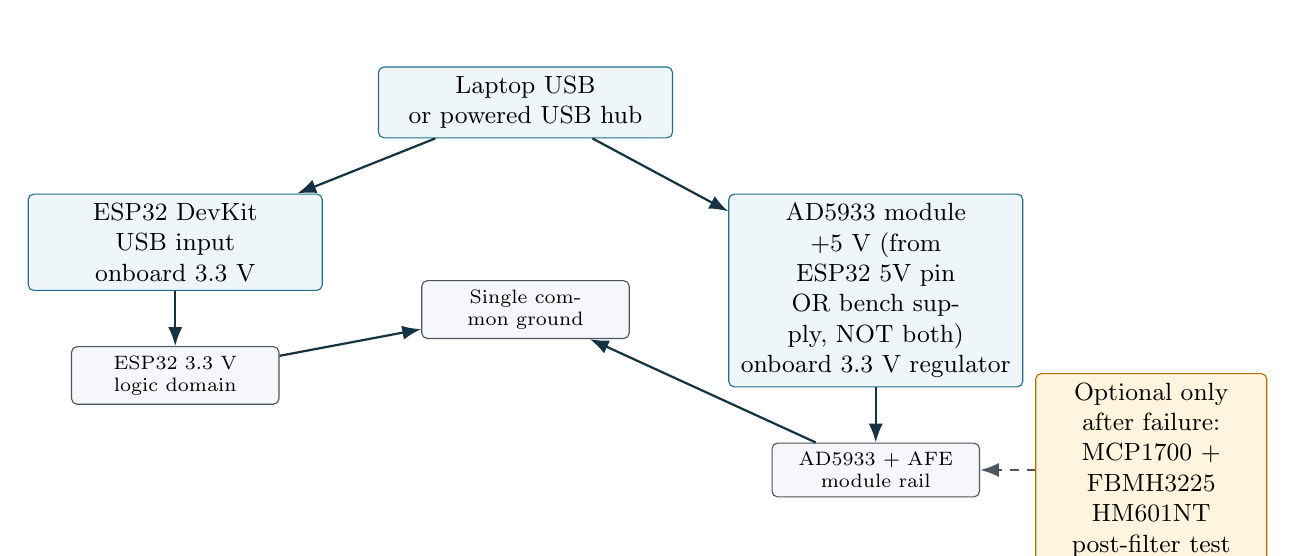
\begin{tikzpicture}[node distance=7mm and 7mm]
\node[eisblockwide] (usb) {Laptop USB\\or powered USB hub};
\node[eisblockwide, below left=of usb] (esp5) {ESP32 DevKit\\USB input\\onboard 3.3 V};
\node[eisblockwide, below right=of usb] (mod5) {AD5933 module\\+5 V (from ESP32 5V pin\\OR bench supply, NOT both)\\onboard 3.3 V regulator};
\node[eissmall, below=of esp5] (logic) {ESP32 3.3 V\\logic domain};
\node[eissmall, below=of mod5] (analog) {AD5933 + AFE\\module rail};
\node[eiswarn, right=of analog] (opt) {Optional only\\after failure:\\MCP1700 +\\FBMH3225\\HM601NT\\post-filter test};
\node[eissmall, below=18mm of usb] (gnd) {Single common ground};

\draw[eisarrow] (usb) -- (esp5);
\draw[eisarrow] (usb) -- (mod5);
\draw[eisarrow] (esp5) -- (logic);
\draw[eisarrow] (mod5) -- (analog);
\draw[eisdashed] (opt) -- (analog);
\draw[eisarrow] (logic) -- (gnd);
\draw[eisarrow] (analog) -- (gnd);
\end{tikzpicture}
}
\caption{Power tree. Do not redesign the power system until resistor data show a noise or stability problem.}
\label{fig:power_tree}
\end{figure}

\begin{rulebox}
\textbf{Power discipline rules (frozen):}
\begin{itemize}
\item Use exactly one \SI{5}{\volt} source for the AD5933 module at a time. Either the ESP32 \texttt{5V/Vin} pin or an external bench supply, never both.
\item ESP32 GND and module GND must be bonded \emph{before} $\mathrm{I^2C}$ SDA/SCL is connected.
\item $\mathrm{I^2C}$ SDA/SCL pull-ups go to \SI{3.3}{\volt} only, never to \SI{5}{\volt}. The module's onboard pull-ups (R4, R5 $\approx \kohm{2.2}$) already bias to its own \SI{3.3}{\volt} rail; do not add a second pull-up to the ESP32 \SI{3.3}{\volt} rail unless $\mathrm{I^2C}$ is proven unstable.
\item Before connecting ESP32 $\mathrm{I^2C}$ to the module, measure the module's SDA/SCL idle voltage with a DMM relative to module GND. Expected $\approx \SI{3.3}{\volt}$. If you measure \SI{5}{\volt} or a floating value, stop and diagnose.
\item Do not back-power the module's \SI{3.3}{\volt} header pin from the ESP32 \SI{3.3}{\volt} rail.
\end{itemize}
\end{rulebox}

\subsection{C.3 Analog signal path: Direct mode versus Dual-op-amp mode}

\begin{figure}[!ht]
\centering
\resizebox{\textwidth}{!}{%
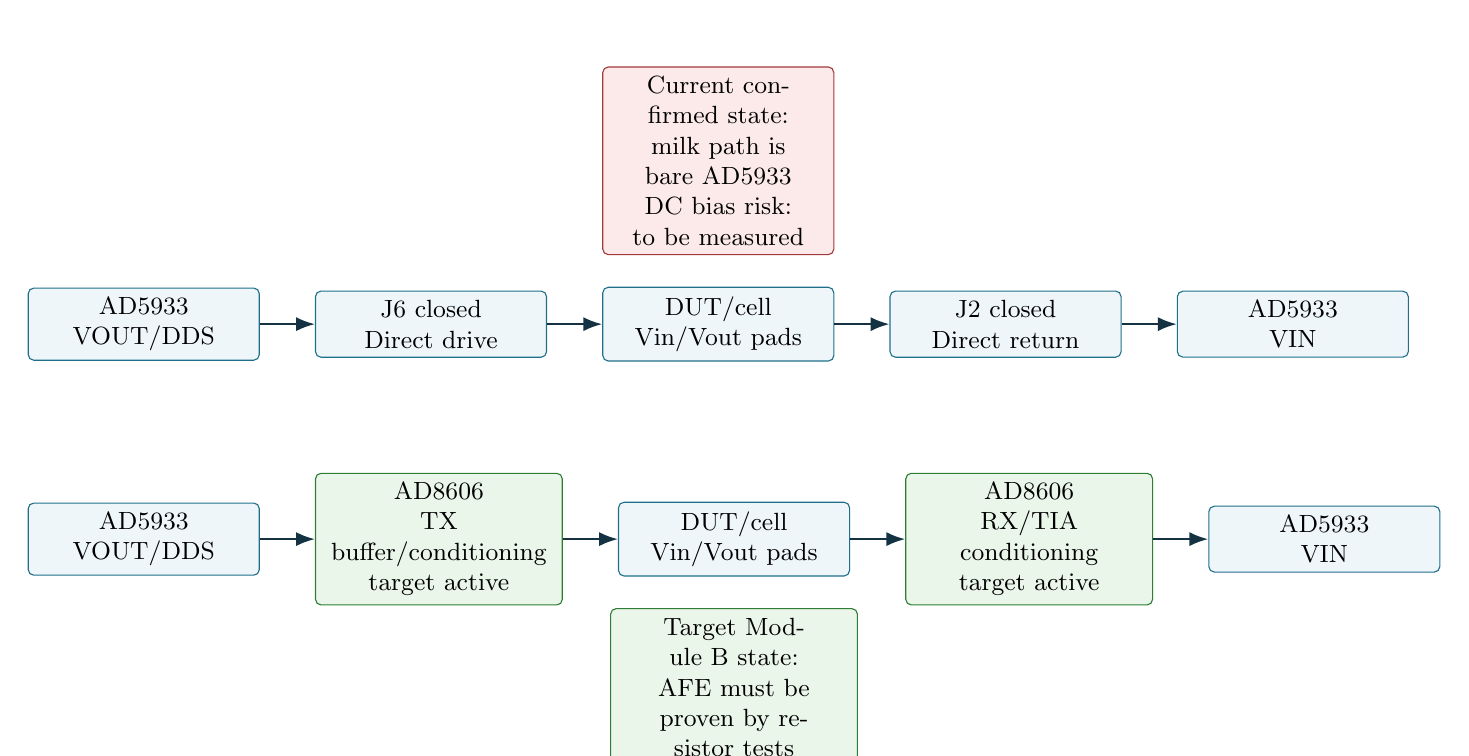
\begin{tikzpicture}[node distance=7mm and 7mm]
\node[eisblock] (dds1) {AD5933\\VOUT/DDS};
\node[eisblock, right=of dds1] (j6) {J6 closed\\Direct drive};
\node[eisblock, right=of j6] (dut1) {DUT/cell\\Vin/Vout pads};
\node[eisblock, right=of dut1] (j2) {J2 closed\\Direct return};
\node[eisblock, right=of j2] (vin1) {AD5933\\VIN};

\node[eisblock, below=18mm of dds1] (dds2) {AD5933\\VOUT/DDS};
\node[eisgreen, right=of dds2] (txafe) {AD8606\\TX buffer/conditioning\\target active};
\node[eisblock, right=of txafe] (dut2) {DUT/cell\\Vin/Vout pads};
\node[eisgreen, right=of dut2] (rxafe) {AD8606\\RX/TIA\\conditioning\\target active};
\node[eisblock, right=of rxafe] (vin2) {AD5933\\VIN};

\node[eisrisk, above=4mm of dut1] (directnote) {Current confirmed state:\\milk path is bare AD5933\\DC bias risk: to be measured};
\node[eisgreen, below=4mm of dut2] (dualnote) {Target Module B state:\\AFE must be proven by resistor tests};

\draw[eisarrow] (dds1) -- (j6);
\draw[eisarrow] (j6) -- (dut1);
\draw[eisarrow] (dut1) -- (j2);
\draw[eisarrow] (j2) -- (vin1);

\draw[eisarrow] (dds2) -- (txafe);
\draw[eisarrow] (txafe) -- (dut2);
\draw[eisarrow] (dut2) -- (rxafe);
\draw[eisarrow] (rxafe) -- (vin2);
\end{tikzpicture}
}
\caption{Analog signal path comparison. The exact vendor AFE transfer function remains open until characterized empirically.}
\label{fig:signal_path}
\end{figure}

\subsection{C.4 Digital/control path}

\begin{itemize}
\item ESP32 $\mathrm{I^2C}$ master at \SI{3.3}{\volt} logic level.
\item The AD5933 7-bit address is \texttt{0x0D}. Arduino \texttt{Wire} library uses 7-bit addressing and expects \texttt{0x0D}. Some vendor code (including the vendor manual page 3) uses the 8-bit shifted form \texttt{0x1A}: do not copy that constant blindly; it is the same device expressed differently.
\item $\mathrm{I^2C}$ clock: start at \SI{100}{\kilo\hertz}; move to \SI{400}{\kilo\hertz} only if \SI{100}{\kilo\hertz} is proven stable and data rate is insufficient.
\item ESP32 reads AD5933 status (\texttt{0x8F}), real (\texttt{0x94}/\texttt{0x95}), imaginary (\texttt{0x96}/\texttt{0x97}), and internal temperature (\texttt{0x92}/\texttt{0x93}) registers.
\item ESP32 reads DS18B20 sample temperature before and after the sweep only.
\item ESP32 sends raw data plus metadata; the laptop computes calibrated impedance.
\item MCLK source: internal (\SI{16.776}{\mega\hertz}) is sufficient for sweeps above $\approx \SI{1}{\kilo\hertz}$. External MCLK is only needed for sub-\SI{1}{\kilo\hertz} work (not required in v1).
\end{itemize}

\subsection{C.5 Calibration and sample paths}

\begin{figure}[!ht]
\centering
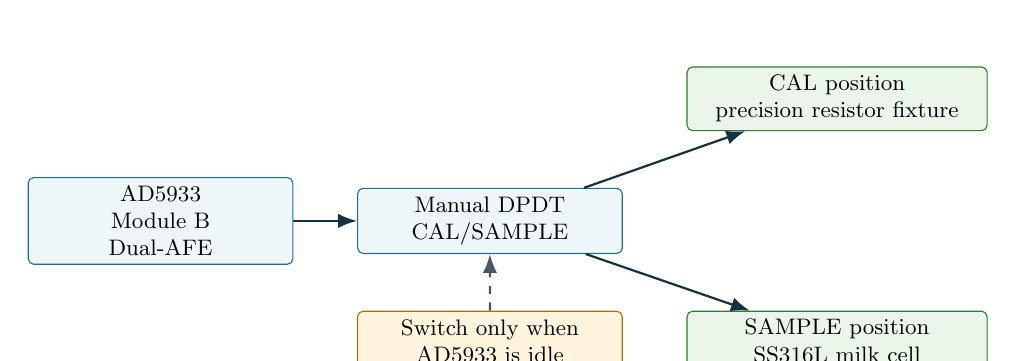
\begin{tikzpicture}[node distance=8mm and 9mm, scale=0.9, transform shape]
\tikzset{
    eisblock/.append style={text width=3.5cm, align=center},
    eisgreen/.append style={text width=4cm, align=center},
    eiswarn/.append style={text width=3.5cm, align=center}
}
\node[eisblock] (ad) {AD5933\\Module B\\Dual-AFE};
\node[eisblock, right=of ad] (switch) {Manual DPDT\\CAL/SAMPLE};
\node[eisgreen, above right=of switch] (res) {CAL position\\precision resistor fixture};
\node[eisgreen, below right=of switch] (cell) {SAMPLE position\\SS316L milk cell};
\node[eiswarn, below=of switch] (rule) {Switch only when\\AD5933 is idle};

\draw[eisarrow] (ad) -- (switch);
\draw[eisarrow] (switch) -- (res);
\draw[eisarrow] (switch) -- (cell);
\draw[eisdashed] (rule) -- (switch);
\end{tikzpicture}
\caption{Manual CAL/SAMPLE switching concept. Switch state is metadata, not a lab note afterthought.}
\label{fig:calsample}
\end{figure}

\subsection{C.6 Fallback path if the module underperforms}

\begin{gatebox}
If Module B in Dual-op-amp mode cannot measure \Rohm{330}, \Rohm{470}, and \kohm{1} within the empirical acceptance thresholds over a contiguous trusted band, do not collect publishable milk data. Fallback sequence: (1)~reduce frequency band; (2)~reduce excitation range; (3)~verify cables and cell; (4)~repeat resistor tests; (5)~compare against Module A Direct mode; (6)~consider external AFE or reference-instrument access.
\end{gatebox}

% ==========================================================================
\section{SECTION D --- Final EIS project BOM/status}
\label{sec:D}

\subsection{D.1 Already available / already bought}

\small
\begin{xltabular}{\textwidth}{L{28mm}L{15mm}L{32mm}L{42mm}Y}
\toprule
\textbf{Name} & \textbf{Qty} & \textbf{Source} & \textbf{Exact version/spec} & \textbf{Project role}\\
\midrule
\endfirsthead
\toprule
\textbf{Name} & \textbf{Qty} & \textbf{Source} & \textbf{Exact version/spec} & \textbf{Project role}\\
\midrule
\endhead

AD5933 impedance-analysis module & 2 & China / Taobao & Shielded AD5933 module with onboard AD8606, +5\,V input, onboard 3.3\,V regulation, $\mathrm{I^2C}$ header, Vin/Vout terminals, DDS-OUT SMA, EXT-CLK SMA, J1--J6 jumper-selectable routing (both confirmed J2+J6 closed = Direct mode) & Core EIS front-end. Module A remains Direct; Module B becomes Dual-AFE candidate.\\
ESP32-DevKitC-32E & 1 & China / Taobao & ESP32-32E DevKit with CH340 USB-UART, 3.3\,V logic & Controller, $\mathrm{I^2C}$ master, 1-Wire temperature reader, USB serial bridge.\\
DS18B20 waterproof temperature probes & 2 & China / Taobao & One imported/Dallas-core, one domestic-core; stainless waterproof probe & Sample temperature before/after sweep; second probe for backup/ambient comparison.\\
Precision resistor set & 10 pcs each value & China / Taobao & 0.1\%, 0.25\,W metal-film; \Rohm{100}, \Rohm{330}, \Rohm{470}, \kohm{1}, \kohm{4.7}, \kohm{10} & Gain/phase calibration, Direct-vs-Dual characterization, trusted-band mapping.\\
47\,nF C0G/NP0 capacitors & 3 & China / Taobao & 1210, 50\,V, C0G/NP0 & Optional analog filtering only.\\
MCP1700-3302E regulators & 3 & China / Taobao & TO-92 3.3\,V LDO & Optional clean 3.3\,V rail contingency.\\
Ferrite beads & 10 & China / Taobao & FBMH3225HM601NT; 1210/3225, $\approx\Rohm{600}$ impedance at \SI{100}{\mega\hertz} (ferrite-bead spec convention) & Optional supply filtering. Replaces refunded Murata BLM31PG601SN1L.\\
SMA solder-head pigtail cables & 2 & China / Taobao & Short SMA male single-head solder, $\approx$\SI{0.1}{\meter} & Usable only as repurposed cable stock; existing module SMAs are DDS-OUT and EXT-CLK, not sample path.\\
FR4 perfboard & 4 & China / Taobao & 5\,cm $\times$ 7\,cm universal perfboard & Semi-permanent wiring carrier after breadboard validation.\\
DPDT toggle switch & 1 & China / Taobao & ETEN 1321 style 6-pin, ON-ON & Manual CAL/SAMPLE switching.\\
Soldering tools and consumables & available & Previous BD purchases / project bench & Iron, solder, flux, wick, tweezers, wires, breadboards, jumpers, DMM & Build, rework, jumper verification, wiring, debug.\\
DMM & 1 & Available (model/accuracy to be logged before GATE~B1) & Used for jumper verification & Continuity, resistor measurement, rail checks, rework validation. Accuracy class must be recorded; it bounds the metrology claim.\\
SS304 stainless sheet & 1 & China / Taobao & 0.5\,mm, 304 & Mechanical mockup only. Excluded from final milk data.\\
\bottomrule
\end{xltabular}
\normalsize

\subsection{D.2 Already ordered / in transit}

\begin{xltabular}{\textwidth}{L{32mm}L{15mm}L{36mm}L{45mm}Y}
\toprule
\textbf{Name} & \textbf{Qty} & \textbf{Source} & \textbf{Exact version/spec} & \textbf{Project role}\\
\midrule
SS316L stainless electrode stock & to confirm & China order, ETA $\approx$ 1--2 weeks & SS316L sheet/strip/foil; size to be logged on arrival & Final electrode material. Must be photographed, measured, cleaned, and logged before first use. Verify authenticity via invoice/certificate.\\
\bottomrule
\end{xltabular}

\subsection{D.3 Still to source locally}

\begin{xltabular}{\textwidth}{L{34mm}L{15mm}L{32mm}L{45mm}Y}
\toprule
\textbf{Name} & \textbf{Qty} & \textbf{Source} & \textbf{Spec} & \textbf{Project role}\\
\midrule
3D printed cell bodies & 3 identical & IUB FabLab & PETG preferred over PLA (better fat tolerance); single CAD revision & Cell-to-cell reproducibility; fixed electrode positioning.\\
Cell fasteners and seals & set & Local & Stainless screws/nuts, nonconductive spacers, gasket or O-ring & Mechanical repeatability.\\
DI or distilled water & sufficient & Lab/local & For cleaning blanks and rinsing & Blank checks, carryover control.\\
UHT milk baseline samples & multiple batches & Local retail & One brand/fat-class per experiment block; record lot and date & Controlled baseline.\\
Adulterants & as approved & Lab/local & Water dilution first; other adulterants only with supervisor-approved protocol & Controlled concentration series.\\
Pipettes / syringes / graduated cylinders & sufficient & Lab/local & Repeatable volumes; dedicated labeled tools & Sample preparation accuracy.\\
Beakers / sample cups & sufficient & Lab/local & Clean, labeled, repeatable volume & Sample handling.\\
Lint-free wipes / gloves / IPA / mild detergent & sufficient & Lab/local & Clean handling; dairy-protein film removal & Electrode cleaning SOP.\\
Material-authenticity documentation & 1 record & Seller/lab & Seller certificate or invoice wording for SS316L & Publication-strengthening evidence.\\
\bottomrule
\end{xltabular}

\subsection{D.4 Optional or backup only}

\begin{xltabular}{\textwidth}{L{38mm}L{22mm}Y}
\toprule
\textbf{Item} & \textbf{Status} & \textbf{Use condition}\\
\midrule
FNIRSI portable oscilloscope / LCR combo & Not confirmed bought; optional & Would be useful for clock/excitation sanity checks. Do not assume availability.\\
Reference LCR meter / impedance analyzer & Open publication-strengthening item & Strongly improves defensibility. Borrow from IUB lab if possible after Module B works.\\
External MCLK oscillator & Optional future & Needed only if sub-\kohm{1} frequency ($<\SI{1}{\kilo\hertz}$) work is added.\\
Second ESP32 & Optional backup & Useful if primary unit fails.\\
Custom PCB & Future only & Not before repeatable data and frozen analog path.\\
Battery / OLED / enclosure polish & Future only & Presentation polish after measurement system works.\\
\bottomrule
\end{xltabular}

\subsection{D.5 Not needed now}

\begin{rulebox}
Do not spend current build effort on: battery operation, OLED, custom PCB, analog multiplexer, automatic sample switching, mobile app inference, cloud dashboard, through-container capacitive sensing, multi-commodity oil/honey/spice extensions, or SS304 publishable electrodes.
\end{rulebox}

% ==========================================================================
\section{SECTION E --- AD5933 module mode and rework manual}
\label{sec:E}

\subsection{E.1 Confirmed jumper measurements}

\begin{center}
\scriptsize
\begin{tabular}{llllllll}
\toprule
\textbf{Module} & \textbf{J1} & \textbf{J2} & \textbf{J3} & \textbf{J4} & \textbf{J5} & \textbf{J6} & \textbf{Mode}\\
\midrule
Module A & $\approx\Mohm{3}$ open & $\approx\Rohm{0}$ closed & $\approx\Mohm{3}$ open & $\approx\Mohm{3}$ open & $\approx\Mohm{3}$ open & $\approx\Rohm{0}$ closed & Direct\\
Module B & $\approx\Mohm{3}$ open & $\approx\Rohm{0}$ closed & $\approx\Mohm{3}$ open & $\approx\Mohm{3}$ open & $\approx\Mohm{3}$ open & $\approx\Rohm{0}$ closed & Direct\\
\bottomrule
\end{tabular}
\end{center}

\subsection{E.2 Acceptance rule for open vs closed}

\begin{rulebox}
\textbf{Jumper-state classification (updated from earlier draft):}
\begin{itemize}
\item \textbf{Closed:} DMM reads $<\Rohm{1}$ or gives a continuity beep.
\item \textbf{Open:} no continuity beep \emph{and} DMM reads megaohm-scale; a reading of several megaohms on a 20~M$\Omega$ range is acceptable as ``open'' (it reflects DMM input impedance, not a partial bridge). Do \emph{not} require $>\Mohm{10}$.
\item \textbf{Ambiguous:} sub-megaohm non-zero reading or inconsistent reading when probes are repositioned $\rightarrow$ treat as a \textbf{fault}, stop and diagnose.
\end{itemize}
\end{rulebox}

\subsection{E.3 Mode interpretation}

Vendor manual \cite{vendorManual}:
\begin{itemize}
\item \textbf{Direct mode:} J2 and J6 closed; J1, J3, J4, J5 open.
\item \textbf{Dual-op-amp mode:} J1, J3, J4, J5 closed; J2 and J6 open.
\end{itemize}
Both purchased modules are confirmed Direct mode. Any earlier claim that the boards probably shipped in Dual-op-amp mode is rejected.

\subsection{E.4 Why this matters for low-impedance milk EIS}

AD5933 data sheet \cite{ad5933ds}: standard impedance range \kohm{1}--\Mohm{10}; \Rohm{100}--\kohm{1} requires additional circuitry. Milk in a small two-electrode cell typically sits in the hundreds-of-ohms region. Direct mode is the least defensible for that region. Dual-op-amp mode is intended to optimize the signal link via the onboard AD8606, but the gain values and AC coupling must be proven by the resistor set (the vendor does not publish the schematic).

\begin{figure}[!ht]
\centering
\resizebox{0.88\textwidth}{!}{%
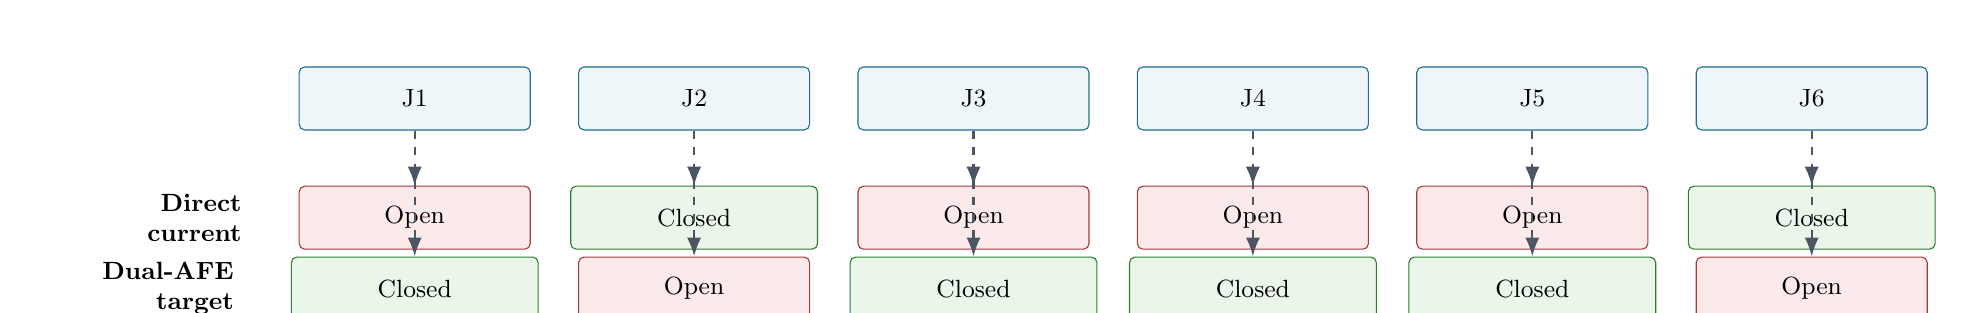
\begin{tikzpicture}[node distance=7mm and 6mm]
\node[eisblock] (j1) {J1};
\node[eisblock, right=of j1] (j2) {J2};
\node[eisblock, right=of j2] (j3) {J3};
\node[eisblock, right=of j3] (j4) {J4};
\node[eisblock, right=of j4] (j5) {J5};
\node[eisblock, right=of j5] (j6) {J6};

\node[eisrisk, below=of j1] (d1) {Open};
\node[eisgreen, below=of j2] (d2) {Closed};
\node[eisrisk, below=of j3] (d3) {Open};
\node[eisrisk, below=of j4] (d4) {Open};
\node[eisrisk, below=of j5] (d5) {Open};
\node[eisgreen, below=of j6] (d6) {Closed};

\node[eisgreen, below=16mm of j1] (u1) {Closed};
\node[eisrisk, below=16mm of j2] (u2) {Open};
\node[eisgreen, below=16mm of j3] (u3) {Closed};
\node[eisgreen, below=16mm of j4] (u4) {Closed};
\node[eisgreen, below=16mm of j5] (u5) {Closed};
\node[eisrisk, below=16mm of j6] (u6) {Open};

\node[align=right, left=6mm of d1, font=\small\bfseries, text width=25mm] {Direct\\current};
\node[align=right, left=6mm of u1, font=\small\bfseries, text width=25mm] {Dual-AFE\\target};

\foreach \a/\b in {j1/d1,j2/d2,j3/d3,j4/d4,j5/d5,j6/d6,j1/u1,j2/u2,j3/u3,j4/u4,j5/u5,j6/u6}
\draw[eisdashed] (\a) -- (\b);
\end{tikzpicture}
}
\caption{Jumper mode diagram. Module B must move from the top row to the bottom row.}
\label{fig:jumper_mode}
\end{figure}

\subsection{E.5 Exact rework table for Module B}

\begin{xltabular}{\textwidth}{L{25mm}L{32mm}L{34mm}Y}
\toprule
\textbf{Jumper} & \textbf{Current state} & \textbf{Target state} & \textbf{Action}\\
\midrule
J1 & Open & Closed & Add solder bridge.\\
J2 & Closed & Open & Remove bridge with wick/flux.\\
J3 & Open & Closed & Add solder bridge.\\
J4 & Open & Closed & Add solder bridge.\\
J5 & Open & Closed & Add solder bridge.\\
J6 & Closed & Open & Remove bridge with wick/flux.\\
\bottomrule
\end{xltabular}

\subsection{E.6 Module labels}

\begin{itemize}
\item \textbf{Before rework}, label both boards on the back side, away from analog traces:
  \begin{itemize}
  \item \texttt{AD5933-A-DIRECT}
  \item \texttt{AD5933-B-DIRECT-PRE-REWORK}
  \end{itemize}
\item \textbf{After successful rework and DMM verification}, relabel Module B as \texttt{AD5933-B-DUAL-AFE}.
\end{itemize}

\subsection{E.7 Exact solder rework procedure}

\begin{enumerate}
\item Clear the bench. Use clean paper or an ESD-safe surface. Photograph Module B before rework (all six jumpers plus full board shots).
\item Disconnect all power, USB, ESP32 wires, probes, and sample wiring. The board must be fully unpowered.
\item Verify the pre-rework state one last time with DMM continuity/Ohms mode.
\item Warm the iron to \SIrange{320}{340}{\celsius} (lower end for leaded solder, higher for lead-free). Use a fine chisel or conical tip. Apply flux to J2 and J6.
\item Use solder wick to remove the existing bridges on J2 and J6. Do not scrape the PCB.
\item DMM-check J2 and J6: target state \emph{open} per the acceptance rule in Section~\ref{sec:E}.2 (no beep, megaohm-scale reading).
\item Apply flux to J1, J3, J4, J5. Add small, clean solder bridges with minimum solder.
\item DMM-check J1, J3, J4, J5: target state \emph{closed} ($<\Rohm{1}$ or beep).
\item Clean flux residue with isopropyl alcohol on a cotton swab. Allow to dry fully.
\item Inspect under magnifier or phone macro. Photograph all six jumpers post-rework.
\item Record results in \texttt{hardware/jumper\_state.csv} with a new row tagged \texttt{post\_rework}.
\end{enumerate}

\subsection{E.8 Post-rework DMM truth table}

\begin{xltabular}{\textwidth}{L{25mm}L{55mm}Y}
\toprule
\textbf{Jumper} & \textbf{Target reading} & \textbf{Decision}\\
\midrule
J1 & $<\Rohm{1}$ or continuity beep & Closed; pass.\\
J2 & no beep; megaohm-scale reading & Open; pass.\\
J3 & $<\Rohm{1}$ or beep & Closed; pass.\\
J4 & $<\Rohm{1}$ or beep & Closed; pass.\\
J5 & $<\Rohm{1}$ or beep & Closed; pass.\\
J6 & no beep; megaohm-scale reading & Open; pass.\\
\bottomrule
\end{xltabular}

\subsection{E.9 Rework risks}

\begin{riskbox}
\begin{itemize}
\item Overheating a jumper pad can lift the pad from the substrate.
\item Excess solder can bridge adjacent passives (R1--R8, C1, C5, C10, C11).
\item Flux residue creates leakage in high-impedance nodes.
\item A half-open or cracked joint can pass visually but fail electrically.
\item Reworking both boards destroys the Direct-vs-Dual comparison figure. Do not rework Module~A.
\end{itemize}
\end{riskbox}

\subsection{E.10 What not to touch during rework}

\begin{itemize}
\item Do not touch AD5933 pins.
\item Do not touch AD8606 pins.
\item Do not remove shield-can anchor solder unless absolutely necessary.
\item Do not alter R1--R8, C1, C5, C10, C11, C4/C6/C8/C9, or the SMA connectors.
\item Do not connect milk cell or ESP32 during rework.
\end{itemize}

\subsection{E.11 Post-rework DC-bias verification (three-measurement gate, v4.0b)}

\begin{gatebox}
\textbf{DC-BIAS GATE G-DC3 (MODULE~A AND MODULE~B, BEFORE ANY WET MEASUREMENT)}
\\[2pt]
\textbf{Why three measurements, not one.} The AD5933 receive stage is hard-biased at $V_{DD}/2$ \cite{ad5933ds}, i.e.\ $\approx\SI{1.65}{\volt}$ at $V_{DD}=\SI{3.3}{\volt}$. The transmit stage (VOUT) carries a programmable DC bias that depends on the selected excitation range (Range~1: \SI{1.48}{\volt}, Range~2: \SI{0.76}{\volt}, Range~3: \SI{0.31}{\volt}, Range~4: \SI{0.173}{\volt}). When the unknown impedance is connected directly between VOUT and VIN with no AC-coupling, the differential DC across the load is the difference between these two biases, which is non-zero in every range. Faradaic electrolysis on SS316L electrodes in milk is driven by this \emph{differential} potential; absolute pad voltages relative to GND are diagnostic for understanding why the differential has the value it has. Therefore the gate logs all three values and pass/fail is decided on the differential.
\\[2pt]
\textbf{Procedure.} The DMM is used in DC-volts mode; AC excitation will average out within the DMM's bandwidth. The AD5933 must be in active output state during the measurement, not standby (in standby, the datasheet \cite{ad5933ds} ties VOUT and VIN internally to ground and the test is meaningless).
\begin{enumerate}
\item Power the module at \SI{5}{\volt}. Do not connect any load across P1/P2.
\item Program a single-point sweep at \SI{10}{\kilo\hertz}, Range~4, PGA~\texttimes1, settling 15. Issue \texttt{Initialize with start frequency} then \texttt{Start frequency sweep}; keep the AD5933 actively excited at \SI{10}{\kilo\hertz} (do not exit to standby) for the duration of the DMM reading.
\item \textbf{No-load condition.} Measure and log: $V_{DC}(P1\!-\!\mathrm{GND})$, $V_{DC}(P2\!-\!\mathrm{GND})$, $V_{DC}(P1\!-\!P2)$. Settle the DMM for $\geq\SI{5}{\second}$ per reading.
\item \textbf{Resistive-load condition.} Place a \Rohm{470} 0.1\% precision resistor across P1/P2. Repeat the three measurements. The resistor-loaded measurement is the more important of the two, because the bias state can shift under load (the VOUT source impedance is \Rohm{600} at Range~4 and forms a divider with the load).
\item \textbf{Primary pass criterion:} $|V_{DC}(P1\!-\!P2)| < \SI{50}{\milli\volt}$ in \emph{both} the no-load and \Rohm{470}-loaded conditions.
\item \textbf{Warning band:} $\SI{50}{\milli\volt} \leq |V_{DC}(P1\!-\!P2)| < \SI{100}{\milli\volt}$. Do not collect publishable wet data; investigate. Try a different excitation range and re-run. Common-mode pad voltages (P1\,/\,GND and P2\,/\,GND) above $\sim\SI{100}{\milli\volt}$ each, with low differential, indicate a high common-mode condition that is acceptable for electrolysis but degrades CMRR -- record but proceed.
\item \textbf{Fail criterion:} $|V_{DC}(P1\!-\!P2)| > \SI{100}{\milli\volt}$ in either condition. Do not connect milk. Apply the AC-coupling fallback in the next subsection or use Module~B in Dual-op-amp mode (where the AD8606 establishes a virtual-ground reference for both transmit and receive sides, driving the differential toward zero independently of range selection).
\item Repeat the full procedure at Range~2 and Range~1 for completeness only \emph{after} the Range~4 result is acceptable. Log results to \texttt{hardware/dc\_bias\_check.csv}.
\end{enumerate}
Log columns: \texttt{module\_id}, \texttt{range}, \texttt{condition} (\texttt{NOLOAD} or \texttt{R470}), \texttt{V\_DC\_P1\_GND\_mV}, \texttt{V\_DC\_P2\_GND\_mV}, \texttt{V\_DC\_DIFF\_mV}, \texttt{V\_DD\_V}, \texttt{date}, \texttt{operator}.
\end{gatebox}

\subsubsection*{E.11.a AC-coupling fallback (only if G-DC3 fails)}

\begin{rulebox}
\textbf{If, and only if, G-DC3 fails on a given module:}
\begin{enumerate}
\item Insert an AC-coupling capacitor in series with VOUT \emph{upstream of the DPDT common terminal}, so the same capacitor is in the loop during both calibration (CAL position) and sample measurement (SAMPLE position). This guarantees the per-frequency gain factor mathematically absorbs the capacitor's reactance.
\item \textbf{Sizing rule.} The capacitor reactance at the lowest sweep frequency must be small relative to the lowest expected sample impedance. For milk in the \Rohm{330}--\Rohm{700} range and a 5\,kHz lower trusted band: $X_C = 1/(2\pi f C)$. At $f=\SI{5}{\kilo\hertz}$: $X_C(\SI{1}{\micro\farad})\approx\Rohm{32}$, $X_C(\SI{10}{\micro\farad})\approx\Rohm{3.2}$, $X_C(\SI{47}{\micro\farad})\approx\Rohm{0.7}$. \textbf{Minimum \SI{10}{\micro\farad} non-polar; \SI{47}{\micro\farad} non-polar/film preferred.} A \SI{1}{\micro\farad} cap is rejected -- at \SI{1}{\kilo\hertz} it injects \Rohm{159}, larger than the SOI impedance.
\item \textbf{Polarity.} Use a non-polar (e.g.\ film, ceramic X7R/C0G with adequate voltage rating, or back-to-back electrolytic). Polarized electrolytics applied to the AD5933 VOUT pin will see polarity reversal with every excitation cycle.
\item \textbf{Recalibrate-through requirement.} Once the cap is installed, all gain-factor and phase-offset calibration runs must be re-done with the cap in place. Old calibration files must be invalidated.
\item \textbf{Trusted-band consequence.} Inserting any AC-coupling cap shifts the reliable lower-frequency limit upward. Verify the resistor characterization at the chosen lower band edge before assuming the cap is benign.
\end{enumerate}
\end{rulebox}

\subsection{E.12 When to stop and ask for help}

Stop immediately if any of the following occurs: pad lifts; bridge spreads to adjacent component; DMM readings are inconsistent across probe repositioning; a jumper reads neither clearly open nor clearly closed; burned smell; component shifted; you feel the urge to ``fix'' an IC pin with a large tip.

% ==========================================================================
\section{SECTION F --- Final build manual from zero to first successful data}
\label{sec:F}

\subsection{F.1 Bench preparation}

\begin{enumerate}
\item Clean bench; remove liquids from the electronics area.
\item Prepare labeled containers: \texttt{Module A Direct}, \texttt{Module B Direct (pre-rework)}, \texttt{calibration resistors}, \texttt{temperature probes}.
\item Create project folders:
\begin{verbatim}
EISight/
  hardware/
    photos/
    jumper_state.csv
    resistor_inventory.csv
    dmm_inventory.csv
    dc_bias_check.csv
  firmware/
  data/
    raw/
    calibration/
    qc/
    features/
  docs/
    lab_notebook.md
\end{verbatim}
\item Start a lab notebook. Every power-up and rework step gets date, operator, hardware ID, result.
\end{enumerate}

\subsection{F.2 Module inspection checkpoints}

For both modules: photograph top/bottom/shield/jumpers/Vin-Vout pads/$\mathrm{I^2C}$ header/SMAs at macro. Confirm no loose solder balls, bent pins, cracked passives, or burned marks. Confirm silkscreen labels (ignore the \texttt{AD5355-EVAL} vendor silkscreen; it is a known vendor error --- the IC under the shield is AD5933 per the sticker and AD8606 topology).

\subsection{F.3 Jumper verification}

\begin{gatebox}
No board may be powered until all six jumpers are DMM-verified and recorded per the acceptance rule in Section~\ref{sec:E}.2.
\end{gatebox}

\subsection{F.4 \textbf{Direct-mode power, $R_{FB}$ inventory, and $\mathrm{I^2C}$ sanity on BOTH modules (before rework, v4.0b)}}

\begin{rulebox}
This step is the most important procedural change in v4.0. Do \textbf{not} rework Module~B until both modules are confirmed functional in their as-received Direct state. Otherwise you cannot distinguish a vendor defect from rework damage. v4.0b adds the $R_{FB}$ inventory measurement (G-RFB) and relaxes the quiescent-current rule from a hard gate to a logged reference.
\end{rulebox}

\textbf{G-RFB (new in v4.0b): on-board $R_{FB}$ inventory.} The Chinese clone module's schematic is unpublished. The on-board feedback resistor connected between AD5933 Pin~4 ($R_{FB}$) and Pin~5 (VIN) determines the transimpedance gain $V_{ADC}=V_{exc}\cdot(R_{FB}/Z_{sample})\cdot G_{PGA}$. The official EVAL-AD5933EBZ default is $R_{FB}=\kohm{200}$ \cite{ug364,ad5933ds}; the Ibba reference design uses selectable values \Rohm{200}, \kohm{2}, \kohm{20}, \kohm{200} \cite{ibba2021}. For a milk impedance of \Rohm{330} at Range~4, $R_{FB}>\kohm{5}$ would saturate the internal ADC. Therefore $R_{FB}$ must be measured before any wet test.

\begin{enumerate}
\item \textbf{G-RFB.} With the module \emph{unpowered}, place the DMM in $\Omega$ mode and measure the resistance between AD5933 Pin~4 and Pin~5 on each module (use a magnifier to identify the pins; on a 16-pin SSOP the spacing is \SI{0.65}{\milli\meter}). If a hard direct probe is impractical, probe the $R_{FB}$ test pad / SMD endpoints instead. Record both modules' values in \texttt{hardware/rfb\_inventory.csv}: \texttt{module\_id, rfb\_measured\_ohm, dmm\_model, date, operator, method (pin-probe / pad-probe)}. \textbf{Safety caution (v4.0c):} a slipped probe on the SSOP package can short adjacent pins or damage the IC. Use fine needle probes, work under magnification, and keep the board fully unpowered. \emph{If safe probing is not achievable at your bench, skip direct RFB probing --- G-SAT (Section~\ref{sec:F}.10) will resolve the saturation question empirically. A skipped G-RFB is not a blocker; a damaged module is.}
\item \textbf{Decide ahead.} Compare the measured $R_{FB}$ to the milk-target window:
\begin{itemize}
\item $R_{FB} \in [\Rohm{330}, \kohm{2}]$: ideal for milk; proceed normally.
\item $R_{FB} \in [\kohm{2}, \kohm{20}]$: borderline; G-SAT (Section~\ref{sec:F}.10) will resolve whether saturation actually occurs at expected milk impedances.
\item $R_{FB} > \kohm{20}$: high probability of ADC saturation at $\Rohm{330}$--$\Rohm{700}$ milk loads; G-SAT is mandatory and a $R_{FB}$-rework path or external buffer (datasheet Fig.~35) should be planned.
\end{itemize}
\item Power Module~A alone via its \texttt{+5V/GND} terminal block from a bench supply or ESP32 5V pin. No $\mathrm{I^2C}$ yet.
\item DMM-measure the \texttt{+3.3V} header pin: expected \SI{3.30 \pm 0.05}{\volt}. Measure quiescent current.
\item \textbf{Quiescent-current rule (relaxed in v4.0b).} \SIrange{15}{25}{\milli\ampere} is a logged reference range, not a hard fail. \textbf{Hard-fail conditions} are: (a) AMS1117 or AD5933 shield rises by $>\SI{15}{\celsius}$ above ambient within \SI{10}{\second} of power-up; (b) $V_{3.3}$ rail drifts by $>\pm 5\%$ or oscillates; (c) Module~A vs Module~B current draw differs by $>50\%$ on identical setup; (d) any visible damage, smell, or audible discharge. If quiescent current is within \SIrange{10}{30}{\milli\ampere} and none of (a)--(d) is observed, proceed.
\item Touch AD5933 shield, AD8606 (U1), AMS1117 (U3) with a finger after \SI{30}{\second}: warm is acceptable; uncomfortably hot is not.
\item Power off. Repeat steps 3--6 for Module~B.
\item Wire ESP32 to Module~A: 5V, GND, SDA$\to$GPIO21, SCL$\to$GPIO22, sharing GND before SDA/SCL.
\item Flash $\mathrm{I^2C}$ scanner. Expected: one device at \texttt{0x0D}.
\item Read STATUS (\texttt{0x8F}) and internal temperature (\texttt{0x92}/\texttt{0x93}) 100 times. Expected: stable bus, temperature between \SIrange{20}{35}{\celsius}. \textbf{Note (v4.0b):} the temperature register stores a 14-bit signed value with D13 as the sign bit and the upper two bits as don't-cares \cite{ad5933ds}; firmware must mask and sign-extend correctly, otherwise sub-zero readings or transient bit flips will appear as nonsense.
\item Plug \kohm{1} resistor across P1/P2. Run a single-point \SI{10}{\kilo\hertz} sweep at Range~4, PGA~\texttimes1, settling~15. Record raw \emph{signed} Re/Im values.
\item Swap to Module~B. Repeat steps 8--11.
\end{enumerate}

\begin{gatebox}
\textbf{GATE F.4 pass criteria:} (i) $R_{FB}$ measured and logged for both modules; (ii) both modules power up cleanly with no hard-fail thermal or rail symptoms; (iii) both respond at \texttt{0x0D}; (iv) 100 consecutive register reads without bus error; (v) both return finite, non-saturated, signed real/imaginary values on a \kohm{1} load at \SI{10}{\kilo\hertz}. \textbf{Only after this gate passes is Module~B reworked.}
\end{gatebox}

\subsection{F.5 Rework Module B}

Perform Section~\ref{sec:E} on Module~B only. Do not rework Module~A. After rework, repeat F.4 steps 5--8 on Module~B to confirm it still powers and communicates.

\subsection{F.6 DC-bias verification}

Perform Section~\ref{sec:E}.11 (DC-BIAS GATE G-DC3, three-measurement procedure) on both modules. Log to \texttt{hardware/dc\_bias\_check.csv} with columns \texttt{module\_id, range, condition, V\_DC\_P1\_GND\_mV, V\_DC\_P2\_GND\_mV, V\_DC\_DIFF\_mV, V\_DD\_V, date, operator}. The \texttt{condition} field is \texttt{NOLOAD} or \texttt{R470}. Pass/fail is decided on $|V_{DC}(P1\!-\!P2)| < \SI{50}{\milli\volt}$.

\subsection{F.7 DMM calibration-resistor metrology}

\begin{enumerate}
\item Record DMM model and accuracy class in \texttt{hardware/dmm\_inventory.csv}.
\item Warm up DMM for 10~min. Record ambient temperature.
\item Null the leads on $\Omega$ mode. Record residual lead resistance.
\item Label all 60 resistors (\texttt{R100\_01} \ldots \texttt{R10k\_10}). Measure each. Record \texttt{nominal\_ohm, measured\_ohm, T\_C, operator, timestamp} in \texttt{hardware/resistor\_inventory.csv}.
\item Remeasure \texttt{R1k\_01} at start/middle/end of session; must agree within DMM accuracy class.
\end{enumerate}

\begin{openbox}
\textbf{DMM accuracy limitation:} the 0.1\% resistors are only as trustworthy as the DMM. If the DMM basic accuracy is worse than 0.1\% (typical handheld DMMs are 0.5\%--1\%), the reported metrology is DMM-limited. Record this honestly in the paper's methods.
\end{openbox}

\begin{gatebox}
\textbf{G-DMMx --- Lab-DMM cross-check on the gain-factor anchor (promoted in v4.0c).}

The per-frequency gain factor is anchored on \texttt{R1k\_01} (and validated on \kohm{1}, \Rohm{470}, \Rohm{330}). Any error in those three measurements propagates through every calibrated $|Z|$ figure in the paper. Therefore, before running the F.10 resistor characterization (and therefore before G-SAT and G-LIN), the three milk-relevant calibration anchors must be cross-checked against the best available reference instrument.
\begin{enumerate}
\item Identify the best DMM accessible at IUB EEE lab (4.5-digit benchtop or better preferred; 6.5-digit ideal).
\item Cross-measure \texttt{R1k\_01}, \texttt{R470\_01}, \texttt{R330\_01} on that meter.
\item Log the readings and the meter's accuracy class to \texttt{hardware/resistor\_inventory.csv} as columns \texttt{lab\_dmm\_ohm}, \texttt{lab\_dmm\_model}, \texttt{lab\_dmm\_accuracy\_class\_pct}.
\item \textbf{Pass:} the lab-DMM and handheld-DMM readings agree within the handheld's accuracy class. Use the lab-DMM value as the calibration anchor downstream.
\item \textbf{Fail:} disagreement larger than the handheld's accuracy class indicates the handheld is mis-calibrated; do not use it as the calibration anchor. Either substitute the lab-DMM values or borrow a better handheld before proceeding.
\end{enumerate}
If a lab DMM cannot be borrowed in time, this gate is skipped, and the metrology claim in the paper must be explicitly bounded by the handheld's accuracy class. Skipped G-DMMx is a known publication weakness, not a blocker for v1 bench work.
\end{gatebox}

\subsection{F.8 Perfboard/fixture build}

Breadboard first (temporary); move to perfboard after F.9 passes. Required:

\begin{xltabular}{\textwidth}{L{35mm}L{35mm}Y}
\toprule
\textbf{Signal} & \textbf{ESP32 side} & \textbf{AD5933 module side}\\
\midrule
GND & ESP32 GND (first) & Module GND\\
SDA & ESP32 GPIO21 & Module SDA\\
SCL & ESP32 GPIO22 & Module SCL\\
Module +5\,V & ESP32 5V/Vin pin OR bench supply (NOT BOTH) & Module +5\,V terminal\\
Sample path & not via ESP32 & Vin/Vout to DPDT switch, then CAL fixture or cell\\
DS18B20 data & GPIO4 with 4.7\,k$\Omega$ pull-up to 3.3\,V & (not on module)\\
\bottomrule
\end{xltabular}

\subsection{F.9 Parasitic fixture characterization (new)}

\begin{gatebox}
Before resistor characterization, run the parasitic-fixture suite:
\begin{enumerate}
\item \textbf{Open test:} DPDT in SAMPLE position, cell cables dangling free, no sample. Sweep as in F.10. Record as \texttt{qc/fixture\_open.csv}. Expected: very large $|Z|$ (noisy) at low frequency, dropping at high frequency as cable capacitance dominates. Gate: no NaN/invalid status flags; real/imag not saturated.
\item \textbf{Short test:} DPDT in SAMPLE position, short the cell cables together with a clean copper wire (shortest possible). Sweep. Expected: small $|Z|$ bounded by lead+cable resistance. Record as \texttt{qc/fixture\_short.csv}.
\item \textbf{Cable-motion test:} plug \kohm{1} into CAL. Start a continuous sweep. Gently flex the cell cables and the DPDT wires. Spectra must not shift visibly. If they do, fix routing and strain relief before proceeding.
\item \textbf{Switch-contact test:} actuate DPDT 10 times between CAL and SAMPLE with \kohm{1} plugged into CAL. Resulting $|Z|$ at \SI{10}{\kilo\hertz} must be repeatable to within 1\%.
\end{enumerate}
\end{gatebox}

\subsection{F.10 Resistor calibration and Direct-vs-Dual characterization (v4.0b: with G-SAT and G-LIN)}

\textbf{Default sweep parameters changed in v4.0b.} Per UG-364, p.~19 \cite{ug364}, the AD5933 with the internal \SI{16.776}{\mega\hertz} oscillator exhibits significant DFT spectral leakage below approximately \SI{1}{\kilo\hertz} and degraded accuracy in the \SIrange{1}{5}{\kilo\hertz} band. The initial publication-candidate trusted band is therefore \SIrange{5}{100}{\kilo\hertz} with internal MCLK. The \SIrange{1}{5}{\kilo\hertz} band may be characterized after \SIrange{5}{100}{\kilo\hertz} passes, with explicit annotation; an external \SI{4}{\mega\hertz} MCLK is the optional fallback for that band (Section~\ref{sec:H}.6).

\begin{enumerate}
\item Build a low-leakage resistor CAL fixture with banana-jack or screw terminals at the DPDT CAL position.
\item Sweep order (both modules): \kohm{1} first (anchor for gain factor), then \Rohm{470}, \Rohm{330}, \Rohm{100}, \kohm{4.7}, \kohm{10}. Re-sweep \kohm{1} at the end of the session as a drift check.
\item \textbf{Default sweep parameters (v4.0b):} \SIrange{5}{100}{\kilo\hertz} in 96 steps of \SI{1}{\kilo\hertz}, settling 15 cycles, Range~4, PGA~\texttimes1. Three repeats per resistor.
\item Laptop computes magnitude residual, phase residual, coefficient of variation, saturation flags, and the trusted-band map using the equations in Section~\ref{sec:H}.2.
\item Generate Direct-vs-Dual plots: magnitude error vs frequency, phase residual vs frequency, repeatability CV vs frequency, trusted-band overlay, and a Direct-vs-Dual summary table for \Rohm{330}/\Rohm{470}/\kohm{1}.
\end{enumerate}

\subsubsection*{F.10.a G-SAT --- saturation/clipping characterization (new in v4.0b; clarified in v4.0c)}

\begin{gatebox}
\textbf{Important (v4.0c).} G-SAT is an \emph{analysis} applied to the resistor-sweep dataset already collected in F.10 above. Do not run a separate sweep for G-SAT; the same six-resistor dataset feeds both the calibration map and this saturation check. The same applies to G-LIN below (it consumes the F.10 \Rohm{470} sweep plus one additional Range-2 sweep on \Rohm{470}).
\\[2pt]
\textbf{Why this gate.} For a near-pure resistive load, $|Z|$ is frequency-independent and the per-frequency gain factor times the measured DFT magnitude equals $1/R$ within calibration tolerance. If the receive-stage TIA + ADC is being clipped, the apparent magnitude underestimates the true current, so $\mathrm{GF}\cdot M$ no longer scales as $1/R$ across the resistor set. This is the cleanest empirical detector of saturation when the on-board $R_{FB}$ is unknown.
\\[2pt]
\textbf{Procedure (analysis on F.10 data).}
\begin{enumerate}
\item Use the F.10 sweeps for \Rohm{100}, \Rohm{330}, \Rohm{470}, \kohm{1}, \kohm{4.7}, \kohm{10} (Range~4, PGA~\texttimes1, settling~15, \SIrange{5}{100}{\kilo\hertz}, 3 repeats each).
\item Anchor: choose the \kohm{1} sweep as the gain-factor anchor (per Section~\ref{sec:H}.2).
\item For each other resistor at each frequency, compute the apparent calibrated $|Z|$ and the residual $\varepsilon_R(f) = (|Z_\mathrm{meas}|(f) - R_\mathrm{DMM})/R_\mathrm{DMM}$. Use the lab-DMM-validated $R_\mathrm{DMM}$ values from G-DMMx where available.
\item \textbf{Pass:} For \Rohm{330}, \Rohm{470}, \kohm{4.7} resistors, $|\varepsilon_R(f)| \leq 5\%$ across a contiguous trusted band of $\geq\SI{20}{\kilo\hertz}$ width within \SIrange{5}{100}{\kilo\hertz}. \kohm{10} and \Rohm{100} may show larger residuals at the band edges, especially at low frequencies (\Rohm{100} is below the AD5933's stated native range).
\item \textbf{Fail signature for saturation:} the \Rohm{330}, \Rohm{470} resistors read \emph{high} ($|Z_\mathrm{meas}| > R_\mathrm{DMM}$, $\varepsilon_R > +5\%$) by an amount that grows monotonically as resistance decreases. This is the fingerprint of a clipped sinusoid producing reduced fundamental-frequency DFT magnitude.
\item \textbf{If G-SAT fails:} do not collect milk data on this module. Remediation paths, in order of preference: (a)~try Module~B in Dual-op-amp mode -- the AD8606 may already provide adequate input-side gain reduction; (b)~$R_{FB}$ rework: desolder the on-board $R_{FB}$ component (identified by tracing AD5933 Pin~4 to its associated SMD resistor) and replace with a precision SMD resistor matched to the milk impedance (\Rohm{470}--\kohm{1}); document with photos, update \texttt{hardware/rfb\_inventory.csv}, and re-run G-SAT; (c)~external attenuator + buffer per AD5933 datasheet Fig.~35 \cite{ad5933ds} -- an op-amp (e.g.\ AD8606 spare channel, AD8627, AD820) with a resistor divider on VOUT and a virtual-$V_{DD}/2$ reference; out of scope for the v1 milk experiment but documented as the publication-grade fallback.
\end{enumerate}
\end{gatebox}

\subsubsection*{F.10.b G-LIN --- amplitude-linearity characterization (new in v4.0b; clarified in v4.0c)}

\begin{gatebox}
\textbf{Important (v4.0c).} G-LIN consumes the Range-4 \Rohm{470} sweep already collected in F.10, plus exactly one additional sweep: \Rohm{470} at Range~2. No other new sweeps are required.
\\[2pt]
\textbf{Why this gate.} Standard EIS practice requires the system to be in its linear small-signal regime: the calibrated $|Z|$ of a passive load must be independent of excitation amplitude. If $|Z|$ measured at Range~4 differs from $|Z|$ measured at Range~2 on the same resistor, either the AD5933 is operating non-linearly, the on-board AFE is amplitude-dependent, or there is an unexpected DC-bias-induced effect. Resolving this before milk is a strong publication argument.
\\[2pt]
\textbf{Procedure.}
\begin{enumerate}
\item Anchor: Range-4 sweep on \Rohm{470} from F.10 (already collected).
\item Repeat the \Rohm{470} sweep at Range~2 (\SI{970}{\milli\volt\,pp}, $V_{DC}=\SI{0.76}{\volt}$). Do not run Range~2 if G-DC3 has not also passed at Range~2.
\item Calibrate the Range-2 sweep using a Range-2 \kohm{1} gain factor (computed independently of Range~4: the gain factor is range-dependent because of the different VOUT source impedance, see datasheet Table~17 \cite{ad5933ds}). This requires one additional \kohm{1} sweep at Range~2.
\item \textbf{Pass:} $||Z|_\mathrm{Range2}(f) - |Z|_\mathrm{Range4}(f)| / R_\mathrm{DMM} \leq 2\%$ across the trusted band.
\item \textbf{If G-LIN fails:} the apparent impedance is amplitude-dependent. Investigate before continuing; possible causes include G-SAT failure (clipping), AC-coupling cap not properly absorbed, or a mode-switch artifact. Document and remediate before milk.
\end{enumerate}
\end{gatebox}

\begin{openbox}
\textbf{Settling-cycles guidance:} start at 15 cycles; if the first few frequency points of a fresh sweep disagree with the rest of the sweep by more than repeat CV, increase settling to 30 or 100. Too many settling cycles slow the sweep but rarely hurt accuracy; too few cause the first points to be biased.
\end{openbox}

\subsection{F.11 Cell assembly workflow}

\begin{enumerate}
\item Print three cell bodies from the same CAD revision.
\item Cut three matched SS316L electrode pairs once material arrives. Deburr. Do not scratch active faces.
\item Install electrodes into fixed printed slots.
\item Solder/crimp cables above the liquid line; add strain relief; no exposed solder in milk.
\item Mark fill line and electrode immersion line.
\item Assign cell IDs: \texttt{CELL01}, \texttt{CELL02}, \texttt{CELL03}. Photograph each.
\item Dry-insulation test: DMM between the two electrode leads, cell empty. Expected $>\Mohm{20}$. If $<\Mohm{10}$, diagnose mechanical short.
\end{enumerate}

\subsection{F.12 First dry tests in the cell}

\begin{itemize}
\item \textbf{Open fixture in cell slot:} verify system reports invalid/noisy behavior. Do not treat open data as real impedance.
\item \textbf{Known resistor inserted in cell slot:} verify calibrated result matches actual resistor.
\item \textbf{Cable motion test in cell slot:} repeat F.9 step 3 but with the cell mounted.
\end{itemize}

\subsection{F.13 DI water tests}

DI water is a blank/carryover check, not a calibration standard.

\begin{enumerate}
\item Fill cell to the marked volume.
\item Settle \SI{60}{\second}.
\item Read DS18B20 sample probe.
\item Sweep 3--5 times.
\item Read DS18B20 again.
\item Empty, rinse, repeat.
\end{enumerate}

\begin{gatebox}
\textbf{Pass:} DI blank behavior qualitatively repeatable between fills. \textbf{Fail:} large drift, visible bubbles, cable-position dependence.
\end{gatebox}

\subsection{F.14 Pure milk tests}

\begin{enumerate}
\item One UHT brand, one fat class for the first repeatability test.
\item Mix gently and identically every time; avoid foam.
\item Bring sample into a narrow temperature window.
\item Fill to fixed volume.
\item Remove bubbles from electrode surfaces.
\item Pre-sweep DS18B20.
\item Five repeats without moving the cell.
\item Post-sweep DS18B20.
\item Clean electrodes; run DI blank before the next sample.
\end{enumerate}

\subsection{F.15 Repeatability checks}

\begin{xltabular}{\textwidth}{L{40mm}Y}
\toprule
\textbf{Check} & \textbf{Minimum v1 requirement}\\
\midrule
Within-fill repeatability & Five sweeps of the same milk fill stable over trusted band.\\
Refill repeatability & Empty, clean, refill same milk; spectrum within empirical limits.\\
Cross-session repeatability & Same milk measured on different days with fresh calibration.\\
Cell-to-cell repeatability & Same milk through \texttt{CELL01}--\texttt{CELL03}.\\
Cleaning/carryover & DI blank after milk does not retain milk-like spectrum.\\
\bottomrule
\end{xltabular}

\subsection{F.16 Data logging and file organization}

\begin{verbatim}
data/
  raw/YYYY-MM-DD/session_id/
  calibration/YYYY-MM-DD/session_id/
  qc/YYYY-MM-DD/session_id/
  features/YYYY-MM-DD/session_id/
  models/YYYY-MM-DD/
hardware/
  photos/
  jumper_state.csv
  resistor_inventory.csv
  dmm_inventory.csv
  dc_bias_check.csv
  cell_geometry.csv
  probe_inventory.csv
\end{verbatim}

\subsection{F.17 Go/no-go matrix (v4.0c)}

\begin{xltabular}{\textwidth}{L{38mm}L{45mm}Y}
\toprule
\textbf{Stage} & \textbf{Go criterion} & \textbf{No-go action}\\
\midrule
Jumper verification & Mode matches truth table. & Do not power; inspect.\\
\textbf{G-RFB} (v4.0b) & $R_{FB}$ measured between Pin~4--Pin~5; logged. \emph{Skippable in v4.0c if SSOP probing is unsafe; G-SAT will resolve.} & Use the decision tree in F.4 to route to either G-SAT or rework planning.\\
Power rail test & +5\,V and +3.3\,V plausible and stable; no F.4 hard-fail. & Stop; inspect regulator/wiring.\\
$\mathrm{I^2C}$ sanity & 100 clean reads; \kohm{1} returns sensible \emph{signed} Re/Im. & Fix bus; verify pull-ups; verify int16 parsing.\\
Post-rework sanity (Module~B) & Same as above after rework. & Stop; re-inspect rework.\\
\textbf{G-DC3} (v4.0b) & $|V_{DC}(P1\!-\!P2)| < \SI{50}{\milli\volt}$ under no-load and \Rohm{470}-loaded, at Range~4. Absolute pad voltages logged. & Add AC-coupling cap (\SI{10}{\micro\farad} min, in CAL+SAMPLE paths upstream of DPDT), OR use Module~B Dual-AFE.\\
Parasitic fixture & Open/short/motion/switch acceptable. & Fix cabling/fixture.\\
\textbf{G-DMMx} (NEW v4.0c) & \kohm{1}, \Rohm{470}, \Rohm{330} cross-checked on a benchtop lab DMM; agreement within handheld accuracy class. & If lab DMM unavailable, gate is skipped; metrology claim bounded by handheld accuracy.\\
\textbf{G-SAT} (v4.0b; analysis on F.10 data) & On \Rohm{330}/\Rohm{470}/\kohm{4.7}: $|\varepsilon_R(f)| \leq 5\%$ over $\geq\!\SI{20}{\kilo\hertz}$ band within \SIrange{5}{100}{\kilo\hertz}. & Module~B Dual-AFE; or $R_{FB}$ rework; or external attenuator/buffer.\\
\textbf{G-LIN} (v4.0b; analysis on F.10 data + 1 extra Range-2 sweep) & Range-4 vs Range-2 \Rohm{470}: agreement $\leq 2\%$. & Investigate amplitude dependence before milk.\\
Resistor primary band & \Rohm{330}/\Rohm{470}/\kohm{1} pass thresholds in trusted band. & No milk data; debug AFE/path.\\
DI-water blank & Repeatable. & Fix cleaning/cell/cables.\\
Pure milk repeatability & Stable within and across refills. & No adulteration study.\\
Adulteration session & CAL and pure control both pass same day. & Discard session.\\
\bottomrule
\end{xltabular}

% ==========================================================================
\section{SECTION G --- Final cell design and implementation guidance}
\label{sec:G}

\subsection{G.1 Final recommended cell architecture}

Fixed-geometry two-electrode parallel-plate cell, SS316L electrodes mounted rigidly in a 3D-printed PETG body. Cell is part of the instrument, not a disposable cup.

\begin{openbox}
Geometry below is a v1 candidate, not permanent scientific truth. It is frozen for publication only after parasitic fixture checks, DI-water blanks, pure milk repeatability, and cell-to-cell reproducibility pass.
\end{openbox}

\subsection{G.2 Electrode material}

\begin{itemize}
\item \textbf{Final material:} SS316L.
\item \textbf{SS304 status:} mockup only. Do not mix SS304 and SS316L data.
\item \textbf{Authenticity:} confirm via seller invoice, receipt wording, or certificate; magnet test (austenitic 316L is weakly magnetic at most); soak a small sample in 0.9\% saline for 24~h --- no visible pitting on genuine 316L.
\end{itemize}

\subsection{G.3 v1 candidate electrode dimensions}

\begin{xltabular}{\textwidth}{L{45mm}Y}
\toprule
\textbf{Parameter} & \textbf{v1 candidate}\\
\midrule
Electrode material & SS316L, \SIrange{0.5}{1.0}{\milli\meter} thick.\\
Active wet face & $\approx$ \SI{8}{\milli\meter} wide $\times$ \SI{12}{\milli\meter} immersed height per electrode.\\
Facing-surface gap & \SI{12}{\milli\meter} fixed.\\
Immersion depth control & Printed fill mark and electrode stop; no freehand depth.\\
Sample volume & \SIrange{20}{30}{\milli\liter}; exact volume fixed and logged.\\
Cable connection & Solder/crimp above liquid line; strain relief; no exposed solder in milk.\\
Cell count & Three identical printed cells from one CAD revision.\\
\bottomrule
\end{xltabular}

\begin{openbox}
\textbf{Geometry fallback rule:} if resistor characterization shows Module~B Dual-AFE cannot handle milk loads below $\approx$ \Rohm{500}, adjust cell constant $\kappa = L/A$ \emph{upward} (increase gap, decrease area) to push expected milk impedance into the board's trusted window. This changes cell geometry and resets the dataset --- so decide before data collection begins.
\end{openbox}

\begin{figure}[!ht]
\centering
\resizebox{0.92\textwidth}{!}{%
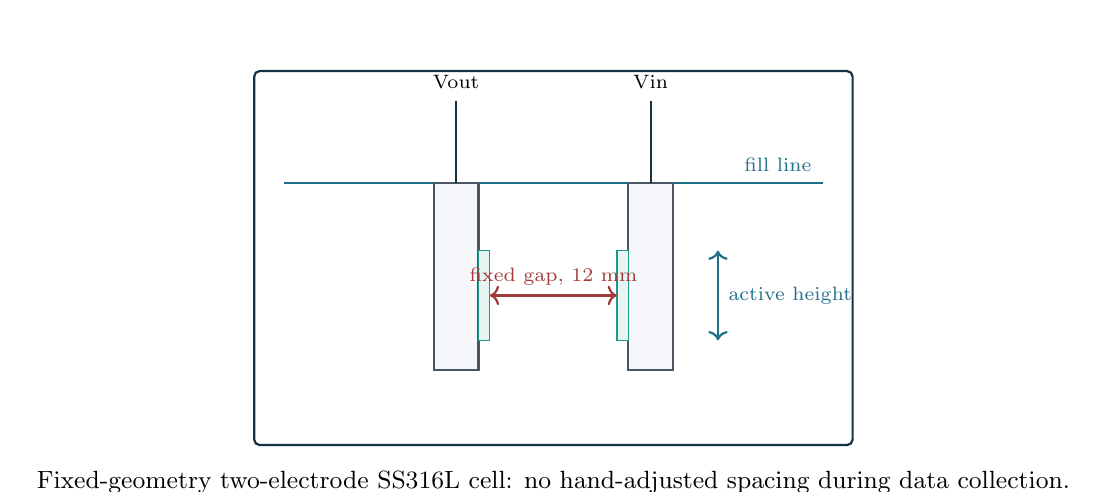
\begin{tikzpicture}[scale=0.95]
\draw[thick, EISNavy, rounded corners=2pt] (0,0) rectangle (8,5);
\draw[thick, EISBlue] (0.4,3.5) -- (7.6,3.5);
\node[font=\scriptsize, EISBlue] at (7.0,3.75) {fill line};
\draw[fill=EISLightGray, draw=EISGray, thick] (2.4,1.0) rectangle (3.0,3.5);
\draw[fill=EISLightGray, draw=EISGray, thick] (5.0,1.0) rectangle (5.6,3.5);
\draw[fill=EISMint, draw=EISTeal] (3.0,1.4) rectangle (3.15,2.6);
\draw[fill=EISMint, draw=EISTeal] (4.85,1.4) rectangle (5.0,2.6);
\draw[<->, thick, EISRed] (3.15,2.0) -- node[above,font=\scriptsize]{fixed gap, 12 mm} (4.85,2.0);
\draw[<->, thick, EISBlue] (6.2,1.4) -- node[right,font=\scriptsize]{active height} (6.2,2.6);
\draw[thick, EISNavy] (2.7,3.5) -- (2.7,4.6);
\draw[thick, EISNavy] (5.3,3.5) -- (5.3,4.6);
\node[font=\scriptsize] at (2.7,4.85) {Vout};
\node[font=\scriptsize] at (5.3,4.85) {Vin};
\node[font=\small, align=center] at (4,-0.5) {Fixed-geometry two-electrode SS316L cell: no hand-adjusted spacing during data collection.};
\end{tikzpicture}
}
\caption{Cell geometry schematic. Dimensions are v1 candidates until repeatability gates pass.}
\label{fig:cell_geometry}
\end{figure}

\subsection{G.4 Cable routing}

\begin{itemize}
\item Keep Vin/Vout leads short ($\le \SI{150}{\milli\meter}$).
\item First tests use short twisted pair. Coax only if shield termination is deliberate.
\item Avoid ground loops through the liquid cell.
\item Mechanical strain relief so cable motion does not move electrodes.
\item Cable route must be identical across cells for cell-to-cell comparison.
\end{itemize}

\subsection{G.5 Mounting strategy}

\begin{itemize}
\item Electrodes slide into printed slots with hard stops.
\item Clamping screws must not bend electrodes.
\item Active area defined by geometry, not by fill-level variation.
\item DS18B20 holder places the probe near sample but not touching electrodes.
\item Cell allows visual bubble inspection.
\end{itemize}

\subsection{G.6 Cleaning strategy}

\begin{enumerate}
\item Immediately after milk, rinse with DI/distilled water.
\item Mild detergent wash if milk film visible or blank fails.
\item Rinse thoroughly with DI.
\item Optional IPA wipe; do not depend on IPA alone for dairy protein.
\item Air dry or lint-free wipe.
\item DI blank before next dataset sample.
\end{enumerate}

\subsection{G.7 Fusion 360 and 3D-printing notes}

\begin{itemize}
\item Parameterize: electrode width, gap, immersion height, fill volume, wall thickness, cable exit angle.
\item Engrave labels: \texttt{CELL01}/\texttt{02}/\texttt{03}, fill line, Vin/Vout side.
\item Print all three in the same orientation and material batch.
\item PETG preferred over PLA (milk fat tolerance).
\item Record slicer settings, material, nozzle size, layer height, print date.
\item Post-process: IPA wipe and \SI{60}{\celsius} DI water soak 30~min $\times$ 3 cycles before first use.
\end{itemize}

\subsection{G.8 Fixed vs adjustable features}

\begin{xltabular}{\textwidth}{L{35mm}L{35mm}Y}
\toprule
\textbf{Feature} & \textbf{Status} & \textbf{Reason}\\
\midrule
Electrode spacing & Fixed & Changes cell constant.\\
Active area & Fixed & Changes cell constant.\\
Immersion depth / fill level & Fixed & Changes interface conditions.\\
Cable strain relief & Fixed during data & Prevents motion artifacts.\\
DS18B20 position & Fixed after validation & Reduces temperature variability.\\
Cell lid/cover & Adjustable for usability & Must not alter electrode geometry.\\
\bottomrule
\end{xltabular}

% ==========================================================================
\section{SECTION H --- Calibration, QC, and measurement protocol}
\label{sec:H}

\subsection{H.1 DMM metrology of calibration resistors}

\begin{enumerate}
\item Label each resistor (\texttt{R330\_01} etc.).
\item DMM-measure after probe stabilization.
\item Record actual value, nominal value, date, operator, DMM model, DMM accuracy class, room temperature.
\item Use the measured values in calibration metadata, not the nominal values.
\end{enumerate}

\begin{openbox}
\textbf{DMM accuracy bound.} Report the metrology limitation honestly in the paper: ``calibration resistors specified at 0.1\% tolerance, DMM-measured on a [model, accuracy class] meter; measurements therefore bounded by DMM accuracy.''
\end{openbox}

\subsection{H.2 Gain and phase calibration (notation corrected)}

At each frequency point $f_i$ the AD5933 returns signed real and imaginary DFT register values, denoted $R_{\mathrm{DFT}}(f_i)$ and $I_{\mathrm{DFT}}(f_i)$. The DFT magnitude is

\begin{equation}
M(f_i) = \sqrt{R_{\mathrm{DFT}}(f_i)^2 + I_{\mathrm{DFT}}(f_i)^2}.
\label{eq:dft_magnitude}
\end{equation}

Let $R_{\mathrm{cal}}$ be the DMM-measured resistance of the calibration resistor. With a near-pure resistive load $Z_{\mathrm{cal}} = R_{\mathrm{cal}}$, the per-frequency gain factor is

\begin{equation}
GF(f_i) = \frac{1}{R_{\mathrm{cal}}\, M_{\mathrm{cal}}(f_i)}.
\label{eq:gain_factor}
\end{equation}

For an unknown sample, the calibrated impedance magnitude is

\begin{equation}
|Z_{\mathrm{unk}}(f_i)| = \frac{1}{GF(f_i)\, M_{\mathrm{unk}}(f_i)}.
\label{eq:unknown_impedance}
\end{equation}

The raw DFT phase is

\begin{equation}
\phi_{\mathrm{raw}}(f_i) = \operatorname{atan2}\!\left( I_{\mathrm{DFT}}(f_i),\, R_{\mathrm{DFT}}(f_i) \right).
\label{eq:raw_phase}
\end{equation}

A near-ideal calibration resistor has zero impedance phase. The measured resistor DFT phase is therefore treated as the system phase offset:

\begin{equation}
\phi_{\mathrm{system}}(f_i) = \operatorname{atan2}\!\left( I_{\mathrm{DFT,cal}}(f_i),\, R_{\mathrm{DFT,cal}}(f_i) \right).
\label{eq:system_phase}
\end{equation}

The corrected sample phase is

\begin{equation}
\phi_{\mathrm{sample}}(f_i) = \operatorname{atan2}\!\left( I_{\mathrm{DFT,sample}}(f_i),\, R_{\mathrm{DFT,sample}}(f_i) \right) - \phi_{\mathrm{system}}(f_i).
\label{eq:corrected_phase}
\end{equation}

If reported in degrees, convert after correction:

\begin{equation}
\phi_{\mathrm{sample,deg}}(f_i) = \phi_{\mathrm{sample}}(f_i)\cdot \frac{180}{\pi}.
\label{eq:phase_deg}
\end{equation}

\begin{rulebox}
\textbf{Phase must be unwrapped} (e.g., with NumPy \texttt{numpy.unwrap}) before any slope, derivative, or Nyquist-arc feature is computed. Raw \texttt{atan2} output has $\pm\pi$ jumps that break downstream analysis.
\end{rulebox}

\begin{openbox}
For milk-range work, prefer a multi-load calibration/validation map rather than a single global gain factor. The calibration resistor should bracket the expected unknown impedance region. For v1, \Rohm{330}/\Rohm{470}/\kohm{1} are the primary milk-relevant calibration/validation loads.
\end{openbox}

\subsection{H.3 Resistor characterization of both modes/modules}

\begin{xltabular}{\textwidth}{L{34mm}Y}
\toprule
\textbf{Load group} & \textbf{Purpose}\\
\midrule
\Rohm{330}, \Rohm{470}, \kohm{1} & Primary milk-relevant acceptance band. Module~B must pass here before milk data.\\
\Rohm{100} & Low-bound stress test.\\
\kohm{4.7}, \kohm{10} & Higher-range characterization.\\
\bottomrule
\end{xltabular}

\subsection{H.4 Empirical acceptance thresholds}

\begin{xltabular}{\textwidth}{L{42mm}L{45mm}Y}
\toprule
\textbf{Metric} & \textbf{Minimum v1 go criterion} & \textbf{Stronger paper target}\\
\midrule
Magnitude residual on primary resistors & $\leq 3\%$ over contiguous trusted band & $\leq 1.5\%$\\
Resistive-load phase residual & $\leq 5^\circ$ over trusted band & $\leq 3^\circ$\\
Within-session CV on resistor magnitude & $\leq 1\%$ & $\leq 0.5\%$\\
Trusted band coverage & At least one contiguous band with enough points for features & Broad, stable band across most planned sweep\\
End-of-session resistor check & Drift $\leq 2\%$ from start check & Drift $\leq 1\%$\\
DC-bias at electrodes & $<\SI{50}{\milli\volt}$ at chosen range & $<\SI{20}{\milli\volt}$\\
\bottomrule
\end{xltabular}

\subsection{H.5 Trusted-band selection (v4.0b: 5--100\,kHz initial candidate)}

\textbf{Initial publication-candidate trusted band: \SIrange{5}{100}{\kilo\hertz} with internal \SI{16.776}{\mega\hertz} MCLK.} The AD5933 internal-oscillator behavior, per UG-364, p.~19 \cite{ug364}, exhibits significant DFT spectral leakage when the excitation period is comparable to or shorter than the 1024-sample DFT window (\SI{977}{\micro\second}). At \SI{1}{\kilo\hertz} (period \SI{1.0}{\milli\second}) the window captures less than one full period, and accuracy degrades. Per-frequency calibration with a known resistor partially absorbs this error but does not eliminate it for non-resistive samples. The conservative ceiling is therefore the \SI{5}{\kilo\hertz} lower bound published in UG-364's Table~2 for the \SI{16}{\mega\hertz} clock.

\textbf{Sub-5\,kHz operation is permitted only after empirical validation:} resistor characterization at the candidate sub-5\,kHz points must show $|\varepsilon_R| \leq 5\%$ on \Rohm{330}/\Rohm{470}/\kohm{1} across $\geq 3$ contiguous frequency points. Any sub-5\,kHz data published from this prototype must be plotted with an explicit annotation (e.g.\ shaded band, footnote citing UG-364) that distinguishes it from the conservative band. The optional fallback is to drive an external \SI{4}{\mega\hertz} MCLK from an ESP32 PWM output into the AD5933 EXT-CLK SMA, with the control register \texttt{0x81[D3]} updated to select external MCLK.

\textbf{A frequency point is in the trusted band only if all of the following hold:}
\begin{itemize}
\item it passes the magnitude residual threshold for \Rohm{330}/\Rohm{470}/\kohm{1} (or a documented justified subset);
\item phase residual is not pathological on resistors;
\item replicate CV is acceptable;
\item AD5933 status flags are valid;
\item no phase discontinuity or saturation appears;
\item G-SAT did not flag the load as clipping at this frequency point.
\end{itemize}

\subsection{H.6 Excitation range and settling cycles (v4.0b: corrected rationale)}

\begin{rulebox}
\textbf{Default for milk v1: Range~4} (\SI{198}{\milli\volt\,pp} AC, \SI{173}{\milli\volt} DC bias on the VOUT pin, \Rohm{600} source impedance \cite{ad5933ds}).

\textbf{Why Range~4 (corrected in v4.0b).} Range~4 minimizes the \emph{AC excitation amplitude} across the load, which is the standard EIS practice for staying in the small-signal linear regime ($V_\mathrm{ac}\!\leq\!\SI{20}{\milli\volt}$ across each electrode is a common literature target; Range~4's \SI{99}{\milli\volt} half-amplitude is acceptable for the milk impedance range we expect). Range~4 does \textbf{not} minimize the differential DC potential $V(P1\!-\!P2)$ across the load when the impedance is connected directly between VOUT and VIN. The receive stage VIN is hard-biased at $V_{DD}/2 \approx \SI{1.65}{\volt}$ \cite{ad5933ds}, so the differential DC across the load is approximately
\[
V_{DC}(P1\!-\!P2) \;\approx\; V_{DD}/2 \;-\; V_\mathrm{VOUT,DC}(\mathrm{range}).
\]
Numerically, at $V_{DD}=\SI{3.3}{\volt}$:

\begin{tabular}{lcc}
\toprule
\textbf{Range} & \textbf{$V_\mathrm{VOUT,DC}$} & \textbf{$V_{DC}(P1\!-\!P2)$ ideal} \\
\midrule
Range~1 & \SI{1.48}{\volt} & $\approx\SI{0.17}{\volt}$ \\
Range~2 & \SI{0.76}{\volt} & $\approx\SI{0.89}{\volt}$ \\
Range~3 & \SI{0.31}{\volt} & $\approx\SI{1.34}{\volt}$ \\
Range~4 & \SI{0.173}{\volt} & $\approx\SI{1.48}{\volt}$ \\
\bottomrule
\end{tabular}

In other words, in raw Direct mode without AC coupling and without the AD8606 buffer, Range~4 actually maximizes the differential DC across the load --- a counter-intuitive result that v4.0 had inverted. The rationale for choosing Range~4 over Range~1 is therefore \emph{linearity, not electrolysis}. Electrolysis is addressed by the G-DC3 gate (Section~\ref{sec:E}.11), which mandates either AC-coupling (E.11.a) or Dual-op-amp-mode buffering (Module~B) to bring the differential below \SI{50}{\milli\volt}, irrespective of range selection.

\textbf{Range escalation rule.} Use Range~4 by default. Escalate to Range~2 only if Range~4 SNR is insufficient \emph{and} the G-DC3 gate also passes at Range~2 \emph{and} G-LIN agreement holds between Ranges 2 and 4. Range~1 (\SI{1.98}{\volt\,pp}) is reserved for resistor characterization in the Direct-mode comparison module only; it is not used for milk.

\textbf{Settling cycles:} default 15; increase to 30 or 100 if first-point bias is observed (per F.10 settling guidance).

\textbf{PGA:} \texttimes1 default; \texttimes5 only after G-SAT confirms there is headroom for the 5$\times$ gain.
\end{rulebox}

\subsection{H.7 Board and sample temperature logging}

\begin{itemize}
\item AD5933 internal temperature register: log as \texttt{ad5933\_temp\_c} (board/die only).
\item DS18B20 sample probe: read before and after sweep only; never during AD5933 conversion.
\item Reject a sweep with $|T_\mathrm{after}-T_\mathrm{before}| > \SI{0.5}{\celsius}$ (early tests may relax this).
\end{itemize}

\subsection{H.8 Sweep QC and rejection rules}

Reject a sweep if any of: missing frequency points; AD5933 status timeout or invalid-data flag; real/imag saturation; phase jump $>10^\circ$ on adjacent resistor points without physical justification; non-physical or negative magnitude; DS18B20 pre/post drift exceeded; CAL check before or after session fails; visible bubbles on electrodes; wrong fill volume; cable moved during sweep; post-milk DI blank fails.

\subsection{H.9 Within-session and cross-session repeatability}

\begin{xltabular}{\textwidth}{L{35mm}Y}
\toprule
\textbf{Test} & \textbf{Protocol}\\
\midrule
Within-session resistor & 5 sweeps per resistor without moving fixture.\\
Within-session milk & 5 sweeps per fill, same milk, no cable/cell movement.\\
Refill & Empty, clean, refill same sample type.\\
Cross-session & Recalibrate on a different day and repeat pure milk.\\
Cell-to-cell & Same milk through \texttt{CELL01}--\texttt{CELL03}.\\
\bottomrule
\end{xltabular}

\subsection{H.10 Contamination/carryover control}

\begin{enumerate}
\item DI blank before first milk sample.
\item Measure pure milk.
\item Clean cell per SOP.
\item DI blank again.
\item If blank contaminated, repeat cleaning; mark preceding sample suspect.
\item Null milk-to-milk (pure-into-pure) check after every third adulterated sample.
\end{enumerate}

\subsection{H.11 Electrode cleaning SOP}

\begin{xltabular}{\textwidth}{L{25mm}Y}
\toprule
\textbf{Step} & \textbf{Action}\\
\midrule
1 & Rinse with DI/distilled water immediately after milk.\\
2 & Gently wash active faces with mild detergent if film visible or blank failed.\\
3 & Rinse thoroughly with DI.\\
4 & Shake dry; wipe with lint-free tissue.\\
5 & Visually inspect for film, spots, bubbles, scratches.\\
6 & DI blank before next dataset sample.\\
\bottomrule
\end{xltabular}

\subsection{H.12 Electrode-polarization warning (new)}

\begin{reviewerbox}
For a two-electrode SS316L cell in milk, low-frequency impedance ($\lesssim \SI{1}{\kilo\hertz}$, sometimes up to a few kilohertz) is typically dominated by electrode polarization at the metal--electrolyte interface, not bulk milk properties. This is a standard reviewer point. State it explicitly in the paper; select the trusted band \emph{above} the polarization region; if necessary, note that a four-electrode geometry (future work) would reduce this effect. The v1 paper claim must be constrained to the trusted band where polarization is small enough.
\end{reviewerbox}

% ==========================================================================
\section{SECTION I --- Software and data architecture}
\label{sec:I}

\subsection{I.1 Pipeline overview}

\begin{figure}[!ht]
\centering
\resizebox{0.96\textwidth}{!}{%
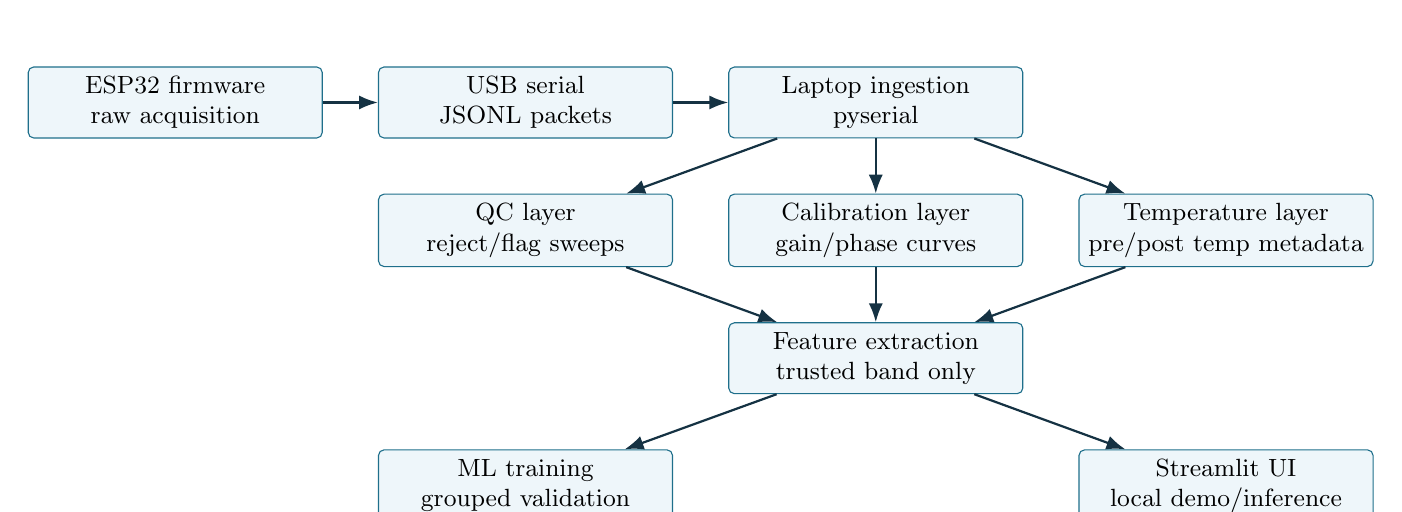
\begin{tikzpicture}[node distance=7mm and 7mm]
\node[eisblockwide] (fw) {ESP32 firmware\\raw acquisition};
\node[eisblockwide, right=of fw] (serial) {USB serial\\JSONL packets};
\node[eisblockwide, right=of serial] (ingest) {Laptop ingestion\\pyserial};
\node[eisblockwide, below=of ingest] (cal) {Calibration layer\\gain/phase curves};
\node[eisblockwide, left=of cal] (qc) {QC layer\\reject/flag sweeps};
\node[eisblockwide, right=of cal] (temp) {Temperature layer\\pre/post temp metadata};
\node[eisblockwide, below=of cal] (feat) {Feature extraction\\trusted band only};
\node[eisblockwide, below left=of feat] (train) {ML training\\grouped validation};
\node[eisblockwide, below right=of feat] (ui) {Streamlit UI\\local demo/inference};

\draw[eisarrow] (fw) -- (serial);
\draw[eisarrow] (serial) -- (ingest);
\draw[eisarrow] (ingest) -- (cal);
\draw[eisarrow] (ingest) -- (qc);
\draw[eisarrow] (ingest) -- (temp);
\draw[eisarrow] (qc) -- (feat);
\draw[eisarrow] (cal) -- (feat);
\draw[eisarrow] (temp) -- (feat);
\draw[eisarrow] (feat) -- (train);
\draw[eisarrow] (feat) -- (ui);
\end{tikzpicture}
}
\caption{Data/software pipeline. Calibration and QC occur before feature extraction.}
\label{fig:data_pipeline}
\end{figure}

\subsection{I.2 ESP32 firmware responsibilities}

\begin{itemize}
\item Initialize $\mathrm{I^2C}$ and AD5933.
\item Configure start frequency, increment, number of increments, settling cycles, excitation range, PGA.
\item Start sweep; poll STATUS (\texttt{0x8F}); read real (\texttt{0x94}/\texttt{0x95}) and imaginary (\texttt{0x96}/\texttt{0x97}) per point.
\item Read AD5933 internal temperature (\texttt{0x92}/\texttt{0x93}) before and after sweep.
\item Read DS18B20 before and after sweep only.
\item Stream raw data plus metadata as JSONL.
\item Watchdog: if sweep-complete status does not appear within expected time, soft-reset AD5933 and report error.
\end{itemize}

\subsubsection*{I.2.a Signed register parsing (frozen rule, v4.0b)}

\begin{rulebox}
The AD5933 stores DFT real (\texttt{0x94}/\texttt{0x95}) and imaginary (\texttt{0x96}/\texttt{0x97}) results in twos-complement 16-bit format \cite{ad5933ds}. The internal temperature register (\texttt{0x92}/\texttt{0x93}) is 14-bit signed; D13 is the sign bit; the upper two bits are don't-cares. Firmware must read MSB and LSB as separate bytes, combine them, and interpret as \texttt{int16\_t} (not \texttt{uint16\_t}). The signed integers are streamed directly in the JSONL \texttt{data} record; the ESP32 does not compute magnitude/phase. The Python ingestion layer must range-validate incoming \texttt{real} and \texttt{imag} values against $[-32768,+32767]$ and refuse any record outside that range. Phase is unwrapped (\texttt{numpy.unwrap}) before any slope or derivative feature. A firmware regression test must exercise both branches -- a known small-negative real component (e.g.\ a capacitive load at high frequency) and a known small-positive real component -- to confirm sign handling.
\end{rulebox}

Reference C/C++ implementation:
\begin{verbatim}
// Real / imag: full 16-bit signed
int16_t real_val = (int16_t)(((uint16_t)real_msb << 8) | real_lsb);
int16_t imag_val = (int16_t)(((uint16_t)imag_msb << 8) | imag_lsb);

// Internal temperature: 14-bit signed in 16-bit envelope
uint16_t raw = ((uint16_t)temp_msb << 8) | temp_lsb;
int16_t  s14 = (int16_t)(raw & 0x3FFF);
if (s14 & 0x2000) s14 -= 0x4000;       // sign-extend D13
float t_c = s14 * 0.03125f;            // 1/32 degC per LSB
\end{verbatim}

Reference Python ingestion:
\begin{verbatim}
def parse_ri(msb, lsb):                # for real and imag registers
    return int.from_bytes(bytes([msb, lsb]), 'big', signed=True)

assert -32768 <= real_val <= 32767     # range guard at ingest
\end{verbatim}

\subsection{I.3 What ESP32 must not do in v1}

\begin{rulebox}
No calibration math, no ML inference, no cloud, no UI. Boring and reliable.
\end{rulebox}

\subsection{I.4 Serial packet format (JSONL)}

\begin{verbatim}
{"type":"hello","fw":"eisight-fw-0.1.0","module_id":"AD5933-B-DUAL-AFE"}
{"type":"sweep_begin","session_id":"2026-04-24_S01",
 "sweep_id":"SWP0001","module_id":"AD5933-B-DUAL-AFE",
 "cell_id":"CAL_FIXTURE","row_type":"CAL","load_id":"R470_03",
 "start_hz":5000,"stop_hz":100000,"points":96,
 "range":"RANGE_4","pga":"X1","settling_cycles":15,
 "ds18b20_pre_c":25.12,"ad5933_pre_c":31.0}
{"type":"data","sweep_id":"SWP0001","idx":0,
 "frequency_hz":5000.0,"real":1234,"imag":-567,"status":2}
{"type":"sweep_end","sweep_id":"SWP0001",
 "ds18b20_post_c":25.14,"ad5933_post_c":31.1,
 "elapsed_ms":1800,"error":null}
\end{verbatim}

\noindent The packet uses the v4.0c default sweep parameters (\SIrange{5}{100}{\kilo\hertz}, 96 steps of \SI{1}{\kilo\hertz}, Range~4). For exploratory sub-5\,kHz characterization runs (Section~\ref{sec:H}.5), use \texttt{start\_hz} as low as \SI{1000}{\hertz} and adjust \texttt{points} accordingly, and tag the row in \texttt{row\_type} or \texttt{notes} as \texttt{LFEXPLORATORY} so downstream QC can separate it from publication-band data.

\subsection{I.5 Raw CSV schema}

\begin{xltabular}{\textwidth}{L{42mm}Y}
\toprule
\textbf{Column} & \textbf{Description}\\
\midrule
session\_id & Date/session identifier.\\
sweep\_id & Unique sweep ID.\\
row\_type & \texttt{CAL}, \texttt{SAMPLE}, \texttt{BLANK}, \texttt{CONTROL}, \texttt{OPEN}, \texttt{SHORT}.\\
module\_id & \texttt{AD5933-A-DIRECT} or \texttt{AD5933-B-DUAL-AFE}.\\
cell\_id & CAL fixture or cell ID.\\
sample\_id & Sample identifier.\\
load\_id & Resistor ID for calibration rows.\\
frequency\_hz & Frequency point.\\
real\_raw & Signed DFT real register value.\\
imag\_raw & Signed DFT imaginary register value.\\
status & AD5933 STATUS register.\\
range\_setting & AD5933 excitation range.\\
pga\_setting & PGA setting.\\
settling\_cycles & Programmed settling cycles.\\
ds18b20\_pre\_c & Sample temperature before sweep.\\
ds18b20\_post\_c & Sample temperature after sweep.\\
ad5933\_pre\_c & AD5933 die temperature before sweep.\\
ad5933\_post\_c & AD5933 die temperature after sweep.\\
operator & Operator initials.\\
notes & Anomaly note.\\
\bottomrule
\end{xltabular}

\subsection{I.6 Calibration CSV schema}

\begin{xltabular}{\textwidth}{L{42mm}Y}
\toprule
\textbf{Column} & \textbf{Description}\\
\midrule
session\_id & Calibration session ID.\\
module\_id & Module used.\\
load\_id & Resistor ID.\\
nominal\_ohm & Nominal value.\\
actual\_ohm & DMM-measured value.\\
dmm\_model & DMM model used for metrology.\\
dmm\_accuracy\_class\_pct & DMM basic accuracy (\%).\\
frequency\_hz & Frequency point.\\
gain\_factor & Per-frequency gain factor.\\
phase\_system\_deg & System phase from resistor.\\
repeat\_cv\_percent & Repeatability CV.\\
trusted\_flag & Point valid for downstream use.\\
\bottomrule
\end{xltabular}

\subsection{I.7 Feature table schema}

\begin{xltabular}{\textwidth}{L{42mm}Y}
\toprule
\textbf{Column} & \textbf{Description}\\
\midrule
sample\_id & Sample identifier.\\
sweep\_id & Source sweep.\\
session\_id & Session.\\
day\_group & Day grouping for validation.\\
brand\_group & Milk brand group.\\
cell\_id & Cell ID.\\
label & Pure/adulterated/concentration label.\\
trusted\_band\_start\_hz & Lower bound of accepted band.\\
trusted\_band\_stop\_hz & Upper bound of accepted band.\\
zmag\_mean, zmag\_slope, phase\_mean, phase\_slope, f\_c & Spectral features.\\
nyquist\_area & Area-like feature on trusted band.\\
qc\_pass & Sweep-level QC boolean.\\
reject\_reason & Empty if accepted.\\
\bottomrule
\end{xltabular}

\subsection{I.8 Firmware/software milestone order}

\begin{enumerate}
\item $\mathrm{I^2C}$ scanner.
\item AD5933 register read/write.
\item Short single-frequency test.
\item Full sweep.
\item DS18B20 read before/after.
\item JSONL serial output.
\item Laptop ingestion and raw logging.
\item Calibration table generation.
\item QC/rejection rules.
\item Parasitic fixture analysis helpers.
\item Trusted-band feature extraction.
\item Streamlit dashboard.
\item ML training with grouped validation.
\item Optional live-inference mode for demo.
\end{enumerate}

% ==========================================================================
\section{SECTION J --- Research audit and publication plan}
\label{sec:J}

\subsection{J.1 Strengths} Strong national relevance; correct scope pivot to milk-first; real inspected hardware; appropriate calibration resistor set; Direct-vs-Dual module comparison as instrumentation figure; laptop-side pipeline allows rigorous QC.

\subsection{J.2 Weaknesses} No validated impedance data yet; no reference instrument comparison; no proven SS316L cell; no confirmed trusted band; no empirical temperature correction; no blind validation; synthetic ML performance is not evidence.

\subsection{J.3 Likely reviewer attacks}

\begin{reviewerbox}
\begin{enumerate}
\item ``How do you know the AD5933 is accurate in milk's impedance range?''
\item ``Where is the reference-instrument comparison?''
\item ``Does the model detect adulteration or just day/brand/temperature drift?''
\item ``Why two electrodes instead of four? How do you handle polarization?''
\item ``What is the DC bias at the electrodes? Are you electrolyzing your sample?''
\item ``How did you control electrode fouling and bubbles?''
\item ``Are repeated sweeps leaking between train and test?''
\item ``What is the limit of detection and uncertainty?''
\item ``What is novel beyond an already published EIS+ML concept?''
\end{enumerate}
\end{reviewerbox}

\subsection{J.4 Mandatory experiments}

\begin{xltabular}{\textwidth}{L{42mm}Y}
\toprule
\textbf{Experiment} & \textbf{Why mandatory}\\
\midrule
Direct-mode sanity (both boards) & Proves hardware works before rework attribution.\\
Resistor characterization, Module~A vs B & Proves analog mode choice and trusted band.\\
DC-bias gate at electrodes & Proves no electrolysis risk.\\
Parasitic fixture (open/short/motion/switch) & Isolates cable/switch artifacts.\\
Pure milk within-session repeatability & Proves the sensor measures a stable liquid.\\
Pure milk cross-session repeatability & Proves calibration/cleaning survive days.\\
DI-water blank/carryover & Proves cleaning is not fiction.\\
Water-dilution series & Safest first adulteration model.\\
Blind holdout samples & Prevents overfitted demo.\\
Cell-to-cell reproducibility & Printed cell is not a one-off artifact.\\
Temperature perturbation subset & Quantifies temperature sensitivity.\\
\bottomrule
\end{xltabular}

\subsection{J.5 Defensible novelty claim}

\begin{quote}
This study presents a low-cost, calibration-audited AD5933/ESP32 milk-EIS prototype with explicit hardware-mode validation (Direct vs Dual-op-amp), DC-bias verification at the electrodes, SS316L fixed-geometry cell design, session-wise calibration, sweep QC, and grouped ML validation for controlled milk-adulteration screening.
\end{quote}

Do not claim: first EIS milk detector; universal food adulteration platform; field-ready deployment; clinical-grade accuracy; smartphone/TinyML/cloud device unless implemented; high accuracy from synthetic data.

\subsection{J.6 Minimum / stronger / journal versions}

\textbf{Minimum publishable:} Module~A vs Module~B resistor characterization; one SS316L cell; one brand; water dilution; $\geq 3$ measurement days; session-wise calibration; day-grouped validation.

\textbf{Stronger conference:} three printed cells; multiple brands; blind samples; reference-LCR cross-check on resistors and subset of liquids; Direct-vs-Dual AFE ablation; temperature ablation; confidence intervals.

\textbf{Journal-oriented:} larger dataset across brands/days/operators/cells; reference-lab validation; formal uncertainty budget; LOD analysis; multiple adulterants; external validation set; long-term drift study; open dataset.

% ==========================================================================
\section{SECTION K --- Risk register and troubleshooting matrix}
\label{sec:K}

\subsection{K.1 Experimental validation ladder}

\begin{figure}[!ht]
\centering
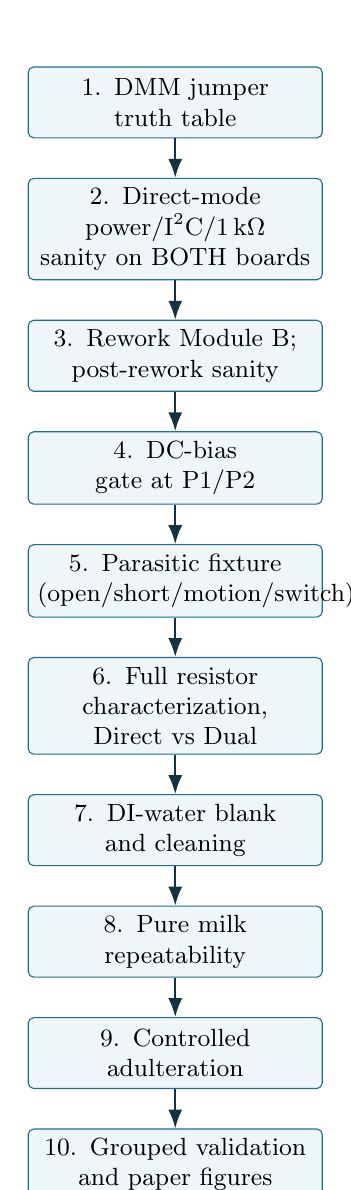
\begin{tikzpicture}[node distance=5mm]
\node[eisblockwide] (l1) {1. DMM jumper truth table};
\node[eisblockwide, below=of l1] (l2) {2. Direct-mode power/$\mathrm{I^2C}$/\kohm{1} sanity on BOTH boards};
\node[eisblockwide, below=of l2] (l3) {3. Rework Module~B; post-rework sanity};
\node[eisblockwide, below=of l3] (l4) {4. DC-bias gate at P1/P2};
\node[eisblockwide, below=of l4] (l5) {5. Parasitic fixture (open/short/motion/switch)};
\node[eisblockwide, below=of l5] (l6) {6. Full resistor characterization, Direct vs Dual};
\node[eisblockwide, below=of l6] (l7) {7. DI-water blank and cleaning};
\node[eisblockwide, below=of l7] (l8) {8. Pure milk repeatability};
\node[eisblockwide, below=of l8] (l9) {9. Controlled adulteration};
\node[eisblockwide, below=of l9] (l10) {10. Grouped validation and paper figures};
\foreach \a/\b in {l1/l2,l2/l3,l3/l4,l4/l5,l5/l6,l6/l7,l7/l8,l8/l9,l9/l10}
\draw[eisarrow] (\a) -- (\b);
\end{tikzpicture}
\caption{Experimental validation ladder (v4.0). Do not skip levels.}
\label{fig:validation_ladder}
\end{figure}

\subsection{K.2 Risk register}

\scriptsize
\begin{xltabular}{\textwidth}{L{26mm}L{31mm}L{29mm}L{31mm}L{18mm}}
\toprule
\textbf{Risk} & \textbf{Likely cause} & \textbf{How to test} & \textbf{Immediate fix} & \textbf{Decision}\\
\midrule
\endfirsthead
\toprule
\textbf{Risk} & \textbf{Likely cause} & \textbf{How to test} & \textbf{Immediate fix} & \textbf{Decision}\\
\midrule
\endhead

Wrong jumper mode & Visual assumption instead of DMM & DMM all six jumpers unpowered & Rework Module~B only & No-go until fixed\\
Vendor-defective board & Dead rail, bad part & Direct-mode power/$\mathrm{I^2C}$ BEFORE rework & Return/replace before rework & No-go\\
Failed rework & Incomplete bridge, lifted pad, short & DMM post-rework, macro photo & Clean/rework if minor; stop if pad risk & Discard data\\
DC bias at electrodes (differential) & No AC cap; raw Direct connection between VOUT bias and VDD/2-biased VIN & G-DC3 three-measurement gate at P1/P2 under active excitation, no-load and \Rohm{470}-loaded & AC-coupling cap (\SI{10}{\micro\farad} min, \SI{47}{\micro\farad} preferred) in CAL+SAMPLE paths, OR Module~B Dual-AFE & Discard wet data until fixed (v4.0b)\\
TIA / $R_{FB}$ saturation (NEW v4.0b) & On-board $R_{FB}$ too large for milk impedance ($R_{FB}/Z \cdot V_\mathrm{exc} > V_{DD}$) & G-RFB inventory + G-SAT resistor sweep & Module~B Dual-AFE; or $R_{FB}$ rework to \Rohm{470}--\kohm{1}; or external attenuator/buffer per datasheet Fig.~35 & No milk data until G-SAT passes\\
Low-frequency DFT spectral leakage (NEW v4.0b) & Internal MCLK + sub-5\,kHz excitation: 1024-sample window does not cover integer periods & Resistor sweep at sub-5\,kHz vs $\geq\!5\,$kHz; check $\varepsilon_R$ & Restrict trusted band to \SIrange{5}{100}{\kilo\hertz}; external \SI{4}{\mega\hertz} MCLK if sub-5\,kHz needed & Flag and exclude sub-5\,kHz unless validated\\
AC-coupling cap calibration leak (NEW v4.0b) & Cap installed in SAMPLE path only, not CAL path & Compare CAL-with-cap vs CAL-without-cap GF & Move cap upstream of DPDT common; full recalibration & Invalidate sessions where mismatch present\\
Unsigned register parsing (NEW v4.0b) & Firmware reads \texttt{0x94}--\texttt{0x97} as \texttt{uint16\_t} & Capacitive-load test; check whether negative-real points appear as $\sim\!65000$ instead of small negative & Update firmware to \texttt{int16\_t} per Section~\ref{sec:I}.2.a; pipeline range-validates ($-32768$..$32767$) & Reprocess raw data; recompute features\\
$\mathrm{I^2C}$ not detected & Wrong address, wiring, pull-up, power, GND & Scanner + DMM rails & Common GND first; 3.3\,V pull-ups & No-go\\
$\mathrm{I^2C}$ pulled to 5\,V by mistake & Pull-up to wrong rail & DMM on SDA/SCL idle & Rewire pull-up to 3.3\,V & Inspect ESP32 pins for damage\\
Unstable Re/Im & Noise, contacts, cable motion & Repeated resistor sweeps & Fix fixture/cables & Discard unstable sweeps\\
\Rohm{330}/\Rohm{470}/\kohm{1} calibration fails & AFE not active, saturation, poor contacts & Primary resistor map & Verify jumpers/range/switch/fixture & No milk data\\
Phase discontinuity & Wrap, SNR, settling & Adjacent-jump rule & Unwrap, increase settling, restrict band & Reject points\\
DMM accuracy insufficient & 0.5\%--1\% handheld DMM & Cross-check on lab DMM & Use best available DMM; state limit & Limit metrology claim\\
Poor DI repeatability & Bubbles, contamination, motion & Repeated blank fills & Improve cleaning, fixed routing & Flag/repeat\\
Pure milk drift & Temperature, creaming, fouling & Repeated pure controls & Standardize timing/temp/clean & No adulteration\\
Electrode polarization dominates & Two-electrode cell, low frequency & Compare bands; review literature & Restrict to higher-frequency band & Constrain claim\\
DS18B20 instability & Pull-up, parasite, water ingress & Dual-probe cup compare & Replace probe & Flag temp data\\
Power/ground noise & Shared supply, long loops & CV vs wiring config & Short ground, powered hub, optional filter & Repeat calibration\\
Sample-path shielding & Long unshielded leads & Cable motion test & Short twisted pair, strain relief & Discard bad\\
Bubbles & Filling/mixing foam & Visual + spectrum jump & Gentle mix, tap, refill & Discard\\
Electrode fouling & Milk protein film & Blank after milk, visual & Cleaning SOP, detergent rinse & Discard sequence\\
Cell geometry drift & Loose slots, hand adjustment & Caliper, repeat same sample & Fix mechanical slots & No-go\\
Unconfirmed SS316L & Seller listing not verified & Invoice; magnet; saline soak & Documentation or mark as assumption & Limit claims\\
No reference instrument & No access to LCR & N/A & Borrow from IUB lab & Weakens paper\\
ML data leakage & Random split across day/brand & Grouped CV vs random split & Rebuild split protocol & Invalidate old metric\\
\bottomrule
\end{xltabular}
\normalsize

\subsection{K.3 Symptom-to-cause troubleshooting table}

\scriptsize
\begin{xltabular}{\textwidth}{L{26mm}L{32mm}L{28mm}L{31mm}L{18mm}}
\toprule
\textbf{Symptom} & \textbf{Likely cause} & \textbf{Test} & \textbf{Fix} & \textbf{Discard data?}\\
\midrule
\endfirsthead
\toprule
\textbf{Symptom} & \textbf{Likely cause} & \textbf{Test} & \textbf{Fix} & \textbf{Discard data?}\\
\midrule
\endhead

Board not detected & Wrong wiring, address, power & $\mathrm{I^2C}$ scan, rail DMM & Rewire, common GND, correct pull-ups & Yes\\
Sweep hangs & Firmware FSM or AD5933 STATUS stuck & Timeout log & Reset AD5933 via STANDBY 0xB0, add watchdog & Yes\\
Re/Im near constant & Wrong register read, no excitation, open path & Known resistor, raw log & Fix firmware/path & Yes\\
Values saturated & Too high signal, wrong range, low load & Sweep \kohm{1}, \Rohm{470} & Lower excitation/PGA, validate AFE & Yes\\
High noise at high freq & Lead parasitics, shielding & Cable motion test & Shorter leads, fixed routing & Usually\\
High noise at low freq & Electrode polarization, settling & Increase settling, compare bands & Restrict band & Affected band\\
Milk spectra shift over minutes & Temperature, creaming, fouling & Temp log, repeat same fill & Fixed timing/mixing/cleaning & Flag/repeat\\
DI blank looks like milk & Carryover and fouling & Repeat after cleaning & Detergent clean, inspect & Yes\\
Module~B worse than Module~A & Rework fault or AFE topology issue & DMM jumpers, resistor map & Inspect/rework or abandon B & Yes for B\\
Direct mode good only at \kohm{1} & AD5933 native range & Compare \Rohm{330}/\Rohm{470} & Use Dual-AFE for milk & Direct not primary\\
ML accuracy unrealistically high & Data leakage by repeat/day/brand & Grouped CV vs random split & Rebuild split protocol & Yes, invalid\\
Electrolysis bubbles on electrode in milk & DC bias leaking through & DMM at P1/P2 under drive & Use Range~4; add series AC cap if needed & Yes\\
\bottomrule
\end{xltabular}
\normalsize

% ==========================================================================
\section{SECTION L --- Required changes from previous blueprint}
\label{sec:L}

Frozen updates to the master blueprint (v3.1 $\rightarrow$ v4.0):

\begin{enumerate}
\item Both AD5933 modules confirmed Direct mode by DMM and visual inspection.
\item AD8606 is present but bypassed in the confirmed current Direct-mode sample path.
\item Module~A remains Direct mode as \texttt{AD5933-A-DIRECT}.
\item Module~B becomes \texttt{AD5933-B-DUAL-AFE} \emph{after} Direct-mode sanity passes on both modules.
\item Any earlier claim that the boards probably shipped in Dual-op-amp mode is rejected.
\item Module SMA connectors are DDS-OUT and EXT-CLK, not the sample Vin/Vout path.
\item Bench-order rule: Direct-mode power/$\mathrm{I^2C}$/\kohm{1} sanity on BOTH modules BEFORE rework.
\item Open-jumper acceptance is ``no beep, megaohm-scale,'' not ``$>\Mohm{10}$.''
\item New \textbf{DC-bias gate} at P1/P2 is mandatory before any wet measurement.
\item New \textbf{parasitic-fixture characterization} (open/short/cable-motion/switch-contact) is mandatory before resistor characterization.
\item Default excitation \textbf{Range~4} for milk contact; Range~1 is forbidden for milk.
\item DMM model and accuracy class recorded in \texttt{hardware/dmm\_inventory.csv}; metrology claim bounded by DMM accuracy.
\item Ferrite-bead spec: FBMH3225HM601NT, $\approx\Rohm{600}$ impedance at \SI{100}{\mega\hertz}.
\item SS316L is the only publishable electrode material; 304 demoted to mockup.
\item Portable oscilloscope is not confirmed bought; optional backup only.
\item DS18B20 sample temperature is read before and after sweep only.
\item Cell geometry remains v1 candidate until repeatability gates pass; geometry fallback rule added if milk $|Z|$ is outside trusted window.
\item Manual CAL/SAMPLE switching frozen for v1.
\item Electrode-polarization warning added explicitly (Section~\ref{sec:H}.12).
\item Phase calibration notation corrected: $R_{\mathrm{DFT}}$ / $I_{\mathrm{DFT}}$ for register values vs $R_{\mathrm{cal}}$ for known resistance; phase unwrap before features.
\item Settling cycles guidance added (start 15, escalate if first-point bias).
\item Grouped validation by day/session/source/cell mandatory.
\item Synthetic ML results are not evidence of physical performance.
\end{enumerate}

\begin{reviewerbox}
The most important correction from earlier drafts is that hardware-mode status is measured, not inferred. DMM continuity is the authority. And rework happens only after Direct-mode sanity confirms vendor delivery was good.
\end{reviewerbox}

\subsection*{L.b v4.0 $\rightarrow$ v4.0b technical patches}

The following patches were applied after a multi-source adjudication (datasheet, UG-364, Ibba 2021, two AI feedback rounds). Patches preserve the v4.0 architecture, BOM, cell, and firmware structure; they tighten the gates between Day-B0 sanity and first-liquid testing.

\begin{enumerate}[leftmargin=1.5em]
\item \textbf{DC-bias gate (Section~\ref{sec:E}.11) is now a three-measurement procedure} (G-DC3): $V_{DC}(P1\!-\!\mathrm{GND})$, $V_{DC}(P2\!-\!\mathrm{GND})$, $V_{DC}(P1\!-\!P2)$. Primary pass on differential $|V(P1\!-\!P2)| < \SI{50}{\milli\volt}$ under both no-load and \Rohm{470}-loaded conditions, under active excitation. Absolute pad voltages retained as diagnostics for common-mode interpretation.
\item \textbf{AC-coupling fallback rule corrected:} minimum \SI{10}{\micro\farad}, preferred \SI{47}{\micro\farad} non-polar/film, placed in series with VOUT \emph{upstream of the DPDT common terminal} so the cap is in both CAL and SAMPLE paths and is absorbed by the per-frequency gain factor. The \SI{1}{\micro\farad} value previously suggested in v4.0 is rejected on the grounds that $X_C(\SI{1}{\kilo\hertz})\!=\!\Rohm{159}$ is comparable to the load.
\item \textbf{$R_{FB}$ inventory gate (G-RFB) added to F.4} (Section~\ref{sec:F}.4): DMM-measure between AD5933 Pin~4 and Pin~5 unpowered; log to \texttt{hardware/rfb\_inventory.csv}. Decision tree on the measured value flags whether saturation is likely.
\item \textbf{Saturation gate G-SAT and amplitude-linearity gate G-LIN added to F.10}, addressing the inferable but unverified TIA/$R_{FB}$ saturation risk for a milk-range load with an unknown clone-module $R_{FB}$. $R_{FB}$ rework is conditional on G-SAT failure, not pre-emptive.
\item \textbf{Trusted-band initial candidate restricted to \SIrange{5}{100}{\kilo\hertz}} (Section~\ref{sec:H}.5), per UG-364 \cite{ug364} guidance on internal-MCLK spectral leakage below ${\sim\,}\SI{5}{\kilo\hertz}$. Sub-5\,kHz operation is permitted only after explicit resistor-QC validation; external \SI{4}{\mega\hertz} MCLK is reclassified as an optional fallback.
\item \textbf{Range~4 rationale corrected (Section~\ref{sec:H}.6):} Range~4 minimizes AC excitation amplitude (linearity-friendly) but does \emph{not} minimize the DC differential across the load when connected directly between VOUT and VIN. Differential is governed by $V_{DD}/2$ on VIN minus $V_\mathrm{VOUT,DC}$. The previous v4.0 wording (``Range~4 minimizes electrolysis'') is corrected.
\item \textbf{Signed int16 register parsing rule (Section~\ref{sec:I}.2.a):} firmware and pipeline must parse \texttt{0x94}/\texttt{0x95} and \texttt{0x96}/\texttt{0x97} as twos-complement 16-bit signed integers, with concrete C and Python examples. Temperature register (\texttt{0x92}/\texttt{0x93}) is 14-bit signed in 16-bit envelope.
\item \textbf{Quiescent-current rule relaxed} (Section~\ref{sec:F}.4): \SIrange{15}{25}{\milli\ampere} is reference, not gate. Hard-fail conditions are explicit (thermal runaway, unstable rail, $>\!50\%$ module mismatch, I\textsuperscript{2}C failure, visible/smell damage).
\item \textbf{Risk register (Section~\ref{sec:K}.2) extended} with five new rows: differential DC-bias, TIA/$R_{FB}$ saturation, low-frequency DFT leakage, AC-cap calibration leak, unsigned register parsing.
\item \textbf{Synthetic Cole--Cole simulation reclassified} as software scaffolding only; no paper figure/metric is sourced from it. (No structural rewrite of the pipeline; only a hygiene rule.)
\end{enumerate}

The patches do \emph{not} require new components, a different cell, or a different ESP32 firmware architecture. The largest operational impact is the trusted-band ceiling at 5\,kHz, which simplifies the initial F.10 sweep and protects the publication argument from spectral-leakage attacks.

\subsection*{L.c v4.0b $\rightarrow$ v4.0c procedural patches}

v4.0c is a small procedural revision following an external review. It adds no new gates and no new components.

\begin{enumerate}[leftmargin=1.5em]
\item \textbf{G-SAT and G-LIN clarified as analyses on the F.10 dataset (Sections~\ref{sec:F}.10.a, \ref{sec:F}.10.b):} both gates are computed from sweeps already collected in F.10 plus, in G-LIN's case, one additional Range-2 \Rohm{470} sweep and its accompanying Range-2 \kohm{1} anchor. They are not separate sweep sessions. This wording change removes the risk of redundant data acquisition.
\item \textbf{G-RFB SSOP-probing safety caution (Section~\ref{sec:F}.4):} a slipped DMM probe on the AD5933 SSOP package can short adjacent pins. If safe probing cannot be achieved, G-RFB may be skipped; G-SAT will resolve the saturation question empirically. A skipped G-RFB is acceptable; a damaged module is not.
\item \textbf{Lab-DMM cross-check promoted to a pre-G-SAT gate (G-DMMx, Section~\ref{sec:F}.7):} the gain factor is anchored on \texttt{R1k\_01} and validated against \kohm{1}/\Rohm{470}/\Rohm{330}, so any handheld-DMM error in those measurements propagates through every calibrated $|Z|$ figure. Cross-check on a benchtop lab DMM before the F.10 resistor characterization. If no lab DMM is available, the gate is skipped and the metrology claim in the paper is bounded by the handheld's accuracy class.
\item \textbf{JSONL example brought into line with the v4.0b default (Section~\ref{sec:I}.4):} \texttt{start\_hz} updated to \SI{5000}{\hertz}, \texttt{points} to 96. Sub-5\,kHz exploratory sweeps must be tagged as such (\texttt{LFEXPLORATORY}) so downstream QC separates them from publication-band data.
\end{enumerate}

% ==========================================================================
\section{SECTION M --- Final action plan}
\label{sec:M}

\subsection{M.1 Next 24 hours (v4.0c)}

\begin{enumerate}
\item Label modules: \texttt{AD5933-A-DIRECT} and \texttt{AD5933-B-DIRECT-PRE-REWORK}.
\item Photograph both modules (top, bottom, shield, jumpers, Vin/Vout, $\mathrm{I^2C}$ header) at macro.
\item Create \texttt{hardware/jumper\_state.csv}, \texttt{dmm\_inventory.csv}, \texttt{rfb\_inventory.csv}, \texttt{dc\_bias\_check.csv}.
\item Re-verify all six jumpers on both modules with DMM; log.
\item Log DMM model and accuracy class in \texttt{dmm\_inventory.csv}.
\item \textbf{G-RFB (new):} DMM-measure $R_{FB}$ between AD5933 Pin~4 and Pin~5 on each module, IC unpowered; log to \texttt{rfb\_inventory.csv}. Apply the decision tree in Section~\ref{sec:F}.4.
\item Power-test Module~A alone: +5\,V input, measure +3.3\,V rail, check heat/current (reference \SIrange{15}{25}{\milli\ampere}; hard-fail criteria per F.4).
\item Power-test Module~B alone (same).
\item Connect ESP32 to Module~A (GND first; SDA/SCL with 3.3\,V pull-ups only). Run $\mathrm{I^2C}$ scanner; confirm \texttt{0x0D}; read STATUS and internal temp 100\texttimes\ \emph{using signed int16 parsing per Section~\ref{sec:I}.2.a}.
\item Repeat step 9 on Module~B.
\item Single-point sweep at \SI{10}{\kilo\hertz}, Range~4, PGA~\texttimes1, 15 settling cycles on \kohm{1} resistor, both modules in Direct mode. Confirm signed Re/Im values are finite and not at $\pm 32767$.
\item \textbf{Only if all above pass}, prepare rework tools and rework Module~B per Section~\ref{sec:E}.
\item Post-rework DMM truth table on Module~B.
\item Post-rework repeat of steps 9--11 on Module~B.
\item \textbf{G-DC3 three-measurement DC-bias gate} (Section~\ref{sec:E}.11) on both modules: log $V_{DC}(P1\!-\!\mathrm{GND})$, $V_{DC}(P2\!-\!\mathrm{GND})$, $V_{DC}(P1\!-\!P2)$ under no-load and \Rohm{470} loaded, at Range~4. Pass on $|V(P1\!-\!P2)| < \SI{50}{\milli\volt}$.
\item Do not connect milk, water, or cell yet.
\end{enumerate}

\subsection{M.2 Next 3 days (v4.0c)}

\begin{enumerate}
\item Implement minimal resistor sweep firmware (JSONL output) with \textbf{signed int16 register parsing} per Section~\ref{sec:I}.2.a. Add a unit test using a capacitive load (\Rohm{1}\,k$\Omega$ + \SI{47}{\nano\farad}) where some imag values must be negative.
\item Laptop ingestion script and raw CSV writer; range-validate signed integers $[-32768, 32767]$ on every record. Default sweep parameters \SIrange{5}{100}{\kilo\hertz}, 96 points, Range~4 (per the v4.0c JSONL example in Section~\ref{sec:I}.4).
\item DMM-measure and label all 60 calibration resistors.
\item \textbf{G-DMMx (v4.0c):} cross-check \texttt{R1k\_01}, \texttt{R470\_01}, \texttt{R330\_01} on the best available IUB lab DMM (per Section~\ref{sec:F}.7). Log to \texttt{resistor\_inventory.csv}.
\item Build clean resistor CAL fixture on perfboard with DPDT.
\item Parasitic-fixture suite (open/short/motion/switch).
\item Begin full resistor characterization at the v4.0c default sweep parameters (\SIrange{5}{100}{\kilo\hertz}, Range~4): \kohm{1} first, then \Rohm{470}, \Rohm{330}.
\item Apply G-SAT and G-LIN \emph{analyses} to the resistor-sweep dataset (no separate sweep sessions). Decide whether $R_{FB}$ rework or external buffer is needed.
\item Compare Module~A Direct and Module~B Dual-AFE on primary resistors.
\item Send advisor email requesting EVAL-AD5933EBZ or reference-LCR loan.
\end{enumerate}

\subsection{M.3 Next 7 days (v4.0c)}

\begin{enumerate}
\item Complete full resistor characterization across all six values on both modules in the trusted band \SIrange{5}{100}{\kilo\hertz}.
\item Optionally extend to \SIrange{1}{5}{\kilo\hertz} if and only if G-SAT/G-LIN both pass at the band edge; explicitly annotate sub-5\,kHz points in the plot.
\item Generate Direct-vs-Dual plots; write the trusted-band selection report including G-SAT/G-LIN evidence.
\item Validate DS18B20 probes (ice-water + room-temp cup compare); assign and log ROM IDs.
\item Design v1 Fusion 360 cell with parameterized electrode geometry.
\item Print first cell body prototype (PETG) in IUB FabLab.
\item Dry-fit assembly using 304 offcut for mechanical check only.
\item Laptop calibration/QC notebook scaffolding.
\end{enumerate}

\subsection{M.4 Next 30 days}

\begin{enumerate}
\item Receive SS316L; document material; cut final electrodes; soak-test in saline for authenticity.
\item Fabricate three identical cells.
\item DI-water blank and cleaning/carryover tests.
\item Pure milk within-session, refill, cross-session, cell-to-cell repeatability.
\item Only after pure milk passes, begin water-dilution adulteration series.
\item Day-grouped validation from first real dataset.
\item Prepare paper figures alongside data: architecture, jumper truth table, DC-bias evidence, resistor validation, trusted band, cell schematic, pure milk repeatability, Direct-vs-Dual comparison.
\item Pre-registration document committed to git before blind-sample decoding.
\item Reference-instrument cross-check on a subset if borrow succeeds.
\end{enumerate}

\begin{verdictbox}
The next real milestone is not an ML accuracy number. It is this: both modules pass Direct-mode sanity, Module~B is reworked and still passes sanity, the DC-bias gate passes, and Module~B in Dual-op-amp mode measures \Rohm{330}, \Rohm{470}, and \kohm{1} repeatably in a documented trusted frequency band. Only then does the milk repeatability work begin. Only after pure milk repeatability does the adulteration study begin.
\end{verdictbox}

% ==========================================================================
\section*{Open items requiring bench clarification or further research}
\addcontentsline{toc}{section}{Open items requiring bench clarification or further research}

The following items are not resolved in this document and are flagged for bench or supervisor resolution:

\begin{enumerate}
\item \textbf{$R_{FB}$ value on the Chinese AD5933 modules (G-RFB, NEW v4.0b).} Vendor schematic is unpublished. Will be settled by the Day-B0 DMM measurement between Pin~4 and Pin~5 on each module, before powering. Determines whether $R_{FB}$ rework or external buffer is required for milk-impedance measurements.
\item \textbf{DC-bias gate outcome (G-DC3).} Whether the module's Direct-mode path contains an AC-coupling capacitor between AD5933 VOUT and P2 is unknown from photographs alone. The three-measurement Day-B0 DMM gate ($P1\!-\!\mathrm{GND}$, $P2\!-\!\mathrm{GND}$, $P1\!-\!P2$, no-load and \Rohm{470}-loaded) settles it.
\item \textbf{Saturation behavior across the resistor set (G-SAT).} Will be characterized by the resistor sweep at \SIrange{5}{100}{\kilo\hertz} on both modules; clipping fingerprint is \Rohm{330}/\Rohm{470} reading systematically high.
\item \textbf{Amplitude-linearity behavior (G-LIN).} Range-2 vs Range-4 \Rohm{470} agreement.
\item \textbf{AD8606 exact topology in Dual-op-amp mode.} The vendor does not publish the schematic. Gain values and TIA feedback must be characterized empirically via the resistor set on Module~B.
\item \textbf{SS316L authenticity.} Chinese order ETA 1--2 weeks; confirm via invoice wording plus magnet test plus 0.9\% saline 24-hour soak.
\item \textbf{DMM accuracy class.} Log the actual meter's basic accuracy and note in the paper; if worse than 0.5\%, a cross-check on an IUB lab DMM is strongly recommended before publication.
\item \textbf{Reference-instrument loan.} Request to Dr.\ Feroz Ahmed for EVAL-AD5933EBZ or benchtop LCR. This is the single highest-leverage item for indexed-conference publication strength.
\item \textbf{Milk impedance actual value.} The v1 candidate cell geometry is designed for 200--700\,$\Omega$ expected milk impedance based on literature; the real value depends on brand, fat, temperature, and our specific cell constant. First pure-milk test answers this; geometry fallback rule (Section~\ref{sec:G}.3) applies if the value lands outside the trusted band.
\item \textbf{Electrode polarization crossover frequency.} Typical two-electrode SS polarization dominates below $\approx\SI{1}{\kilo\hertz}$ but the exact crossover for this cell must be measured. The trusted band will exclude the polarization-dominated region.
\item \textbf{Sub-5\,kHz operability.} Open until the resistor characterization tells us whether per-frequency calibration absorbs the internal-MCLK leakage well enough at \SIrange{1}{5}{\kilo\hertz}, or whether the optional \SI{4}{\mega\hertz} external MCLK must be added.
\item \textbf{Settling-cycles optimum.} Start at 15; will be tuned per module empirically during GATE F.10.
\item \textbf{Blind-sample protocol.} Requires coordination with Mahin or Rafi; pre-registration document drafted before decoding.
\end{enumerate}

\begin{thebibliography}{9}

\bibitem{ad5933ds}
Analog Devices, \textit{AD5933: 1 MSPS, 12-Bit Impedance Converter, Network Analyzer}, Rev.~F, data sheet (project-uploaded).

\bibitem{ug364}
Analog Devices, \textit{UG-364: Evaluating the AD5933 1 MSPS, 12-Bit Impedance Converter Network Analyzer}, evaluation-board user guide (project-uploaded).

\bibitem{vendorManual}
Vendor module document, \textit{AD5933 Impedance Converter Network Analyzer Module User Manual} (project-uploaded). \textbf{Use with caution:} pages 1--5 (mode configuration, jumper logic, I\textsuperscript{2}C addressing, basic register-init sequence) are usable as starter reference; pages 8--9 (marketing copy claiming \SI{10}{\hertz}--\SI{1}{\mega\hertz} sweep, SPI support, anecdotal lab stories) contradict the official data sheet and are disqualified for this project.

\bibitem{auraProgress}
EISight, \textit{AURA Phase 2 Project Progress Report}, project-uploaded progress report.

\bibitem{purchaseAudit}
EISight project record, Taobao purchase audit and uploaded order screenshots.

\bibitem{pipeline}
EISight, \texttt{eisight\_pipeline.py}, project-uploaded source file.

\bibitem{projectUpdate}
EISight hardware update, DMM continuity measurements on both modules (2026-04-24) and uploaded board photographs. Source of truth for jumper state and Direct-mode confirmation.

\bibitem{ibba2021}
P.\ Ibba \emph{et al.}, ``Design and Validation of a Portable AD5933--Based Impedance Analyzer for Smart Agriculture,'' \textit{IEEE Access}, vol.~4, 2021. Reference architecture for AD5933 + AD8606 AFE with selectable $R_{FB}$.

\bibitem{ashoorirad2021}
M.\ Ashoorirad \emph{et al.}, ``Bioimpedance sensor to detect water content in milk based on van der Pauw,'' \textit{IET Nanobiotechnology}, 2021. Reference for milk characteristic frequency ($\approx 23$--$46\,\mathrm{kHz}$) and water-dilution linear trend.

\end{thebibliography}

\end{document}
